% ============================================================
%  Publication 1 — Physics / Quantum Information
%  "Relational Coherence Budgeting for Tunable Exchange Gates:
%   Pointer-Basis Affinity, Decoherence, and Exchange-Angle
%   Coherence Cost"
%
%  SUBMISSION VERSION: Physical Review A (APS)
%  Class: revtex4-2 with [aps,pra,preprint]
%  Compiler: pdflatex (Overleaf)
%  Dr. Joshua Adams | 2026
% ============================================================
%
% NOTES ON THIS VARIANT (read before editing):
%  * REVTeX 4.2 ships with TeX Live / Overleaf / the APS submission
%    system -- unlike sn-jnl.cls (Foundations variant), the class file
%    does NOT need to be bundled in the submission zip. APS compiles it.
%  * "preprint" = one-column, wide-margin, single-spaced-ish REFEREE
%    format, which APS PREFERS for submission (the two-column "reprint"
%    is the published-page look). One-column also means the shared
%    section files' \begin{table}/\begin{figure} do not overflow a
%    column, so NONE of sections/*.tex needs a PRA-specific edit.
%  * apsrev4-2.bst (numbered) matches the plain \cite{} usage already in
%    sections/*.tex -- same reasoning as the Foundations sn-basic choice.
%  * The abstract (sections/00-abstract.tex) is multi-paragraph and
%    contains displayed equations and citations. APS style prefers a
%    single paragraph without displayed math; this compiles as-is, but
%    consider trimming to a single paragraph before final submission.

\documentclass[aps,pra,preprint,amsmath,amssymb,superscriptaddress,nofootinbib]{revtex4-2}
\pdfoutput=1

% ── Encoding & fonts ──────────────────────────────────────
% revtex4-2 sets up fonts; utf8 input is safe to declare.
\usepackage[utf8]{inputenc}
\usepackage[T1]{fontenc}

% ── Mathematics ───────────────────────────────────────────
% revtex4-2 loads amsmath/amssymb via class options above; add the rest.
\usepackage{amsthm}
\usepackage{mathtools}
\usepackage{braket}          % \Bra{}, \Ket{}, \Braket{}
\usepackage{physics}         % \tr{}, \norm{}, \comm{}{}

% ── Quantum circuits ──────────────────────────────────────
\usepackage{quantikz}        % quantum circuit diagrams

% ── Graphics & tables ─────────────────────────────────────
\usepackage{graphicx}
\usepackage{booktabs}        % \toprule/\midrule/\bottomrule -- REVTeX
                             % does NOT load booktabs and, unlike
                             % sn-jnl.cls, does NOT predefine \toprule
                             % etc. under any name, so load the real
                             % package here (no alias hack needed, and
                             % no class-macro collision to worry about).
\usepackage{array}
\graphicspath{{figures/}}

% ── Hyperlinks ────────────────────────────────────────────
% hyperref last. REVTeX is hyperref-aware; colorlinks kept off by
% default for the referee PDF (APS convention), links still active.
\usepackage{hyperref}

% ── ORCID iD in author line ───────────────────────────────
% Loaded AFTER hyperref (and after quantikz, which provides tikz) because
% orcidlink depends on both. Provides \orcidlink{iD}; see author line below.
\usepackage{orcidlink}

% ── Line breaking ─────────────────────────────────────────
% Let TeX loosen a line slightly before letting long inline math
% overflow the margin. Only affects paragraphs that would otherwise
% produce an overfull box.
\setlength{\emergencystretch}{2em}

% ── Custom commands ───────────────────────────────────────
\newcommand{\RCF}{\textsc{rcf}}
\newcommand{\URA}{U_{\!\mathrm{RA}}}
\newcommand{\rhoSE}{\rho_{SE}}

% ── Theorem environments ──────────────────────────────────
\newtheorem{theorem}{Theorem}
\newtheorem{proposition}{Proposition}
\newtheorem{corollary}{Corollary}
\newtheorem{definition}{Definition}
\newtheorem{remark}{Remark}

% =============================================================
\begin{document}
% =============================================================

\title{Relational Coherence Budgeting for Tunable Exchange Gates:
       Pointer-Basis Affinity, Decoherence, and Exchange-Angle
       Coherence Cost}

% ORCID: REVTeX 4.2 provides NO \orcid command of its own (a bare
% \orcid{...} is an undefined-control-sequence error). The documented,
% RevTeX-specific mechanism is the orcidlink package's \orcidlink{iD}
% placed in the author's name argument (orcidlink's own manual uses a
% RevTeX \author line as its worked example). Unlike the Foundations
% variant's \orcidlogo collision, there is no clash here: revtex4-2.cls
% does not define \orcidlink or \orcidlogo, so loading orcidlink is safe.
% orcidlink needs hyperref + tikz; tikz is already pulled in by quantikz
% and hyperref is loaded above, so orcidlink is loaded AFTER both.
% ORCID is ALSO entered in the submission-portal author metadata.
\author{Joshua Adams\,\orcidlink{0000-0002-7185-9125}}
\email{contact@joshuaadams.dev}
\affiliation{Independent Researcher}

\date{\today}

\begin{abstract}
% ── ABSTRACT ──────────────────────────────────────────────────────────────────
% Shared by main.tex (Quantum) and main-pra.tex (PRA). No citations or
% display equations (APS abstract convention). Numbers must match
% Sec. 6.5 / Table and the conclusion: +0.040 (uniform gamma = 0.15),
% +0.025 (heterogeneous gamma in [0.02, 0.30]), E_target = 1, L = 8.

Decoherence theory already explains why system properties become
definite. This paper asks what that explanation is worth to someone who
can tune the strength of an entangling gate. The Relational Coherence
framework (\RCF) restates four standard identities of pointer-basis
coherence theory in terms of a normalized Hilbert--Schmidt quantifier
$\bar\alpha(S,E)\in[0,1]$, fixed by einselection, and treats the drop
$\bar\alpha^{\rm pre}-\bar\alpha^{\rm post}$ across a circuit layer as a
cost. None of this changes the predictions of quantum mechanics.
Rovelli's relational interpretation serves as the conceptual setting;
I do not argue that Bell's theorem singles it out.
For tunable Heisenberg-exchange gates $\URA(\theta)$ under Markovian
dephasing proportional to gate time, with per-layer rates
$\tilde\gamma_\ell$ and a fixed entanglement target
$\sum_\ell|\sin 2\theta_\ell|$, I prove that the cost-minimizing
schedule is unique:
$\theta_\ell^{*}=\tfrac12\arccos[\min(1,\tilde\gamma_\ell/2\lambda^{*})]$,
where the multiplier $\lambda^{*}$ is set by the target. Quiet layers
receive more entanglement, and any layer with
$\tilde\gamma_\ell\ge 2\lambda^{*}$ receives none. In eight-layer
density-matrix simulations with unit target, the schedule improves
final-state fidelity by up to 0.040 over a single full entangler
($\gamma=0.15$) and by 0.025 over equal angles when per-layer noise
ranges from 0.02 to 0.30. The per-gate behavior agrees with published
continuous-fSim results on Sycamore-class processors. These gains
assume the exchange angle can be calibrated directly; where
$\URA(\theta)$ has to be built from fixed native gates, they may shrink
or disappear.

\end{abstract}

\maketitle

% ── Body sections ─────────────────────────────────────────
% ── SECTION 1: INTRODUCTION (~500 words) ──────────────────────────────────────

\section{Introduction}
\label{sec:intro}

Bell's theorem~\cite{Bell1964,CHSH1969} together with its experimental
verification, culminating in the 2022 Nobel Prize in
Physics~\cite{Aspect1982,Zeilinger2022Nobel}, rules out local
non-contextual hidden-variable completions of quantum mechanics.
Several ontologically distinct programmes respond to this constraint:
Bohmian mechanics retains predetermined values at the cost of explicit
nonlocality~\cite{Bohm1980}; many-worlds dispenses with a single outcome
in favour of a universal wavefunction~\cite{Wallace2012}; QBism reads
the quantum state as an agent's degree of belief~\cite{FMS2014}; and
relational quantum mechanics (RQM)~\cite{Rovelli1996,Rovelli2021}
treats quantum properties as facts relative to the interacting systems.

The present paper works within the relational reading, without
claiming that Bell's theorem singles it out among the options above.
What I contribute is an explicit quantitative formulation of one
aspect of the relational picture~--- the dynamics of pointer-basis
coherence under decoherence~--- as a single computable scalar
quantity, the
\emph{scalar affinity} $\bar\alpha(S,E) \in [0,1]$, defined as the
normalized Hilbert--Schmidt coherence of the reduced state $\rho_S$
in the einselected pointer basis~\cite{Zurek2003,Schlosshauer2005}.
The Relational Coherence framework (\RCF) collects four standard
identities involving $\bar\alpha$, suitable as a per-layer
coherence-budget diagnostic in two-qubit circuits.
I stress at the outset that the \RCF~does not dispute the predictive
record of standard quantum mechanics; it offers a unified notation for
relating coherence, decoherence, and entanglement dynamics, and my
mathematical content reduces to standard pointer-basis coherence
theory~\cite{Baumgratz2014,Streltsov2017Review} grounded by einselection.

The \RCF~comprises four propositions: property indefiniteness (a
nonzero $\bar\alpha$ precludes a pointer-basis-diagonal $\rho_S$);
relational determination ($\bar\alpha$ decays exponentially under
Markovian dephasing in the pointer basis); coherence--affinity
correspondence ($\bar\alpha$ ranges continuously over $[0,1]$ with
extrema at full decoherence and the equal-weight pointer-basis
superposition); and coherence redistribution under unitary $S$--$E$
evolution (purity is conserved, mutual information grows, and local
off-diagonals are exported into environment-record orthogonality).
The proofs reduce to Cauchy--Schwarz, a Lindblad calculation, a
Schmidt-decomposition identity, and the Joos--Zeh / Zurek branching
argument~\cite{JoosZeh1985,Zurek2003}, in each case packaged so that
the role of $\bar\alpha$ as a circuit-level figure of merit is
explicit.

Continuously parameterized two-qubit exchange gates are a mature
hardware engineering line: from Loss--DiVincenzo
spin-qubit exchange~\cite{LossDiVincenzo1998}, through parametric
entangling gates on transmon platforms~\cite{Caldwell2018}, to the
continuous fSim/$XY$ families demonstrated on
Sycamore~\cite{Foxen2020,Abrams2020,Lacroix2020} and the
continuously parameterized $\mathcal{ZZ}$ (M\o{}lmer--S\o{}rensen)
gates studied for trapped-ion hardware~\cite{Yale2025NoiseAware}.
Noise-aware compilation exploiting continuous parameterization has
been demonstrated to improve circuit fidelity by routing heavier
entangling weight to better-performing gate pairs and removing
low-impact entangling operations~\cite{Yale2025NoiseAware}.
Building on this literature, I examine the isotropic Heisenberg-exchange
unitary
$\URA(\theta) = \exp[-i\theta(\sigma_x{\otimes}\sigma_x +
\sigma_y{\otimes}\sigma_y + \sigma_z{\otimes}\sigma_z)/2]$,
$\theta \in [0,\pi/2]$, which traces the main diagonal
$(c_1,c_2,c_3)=(\theta,\theta,\theta)$ of the Weyl chamber of
$\mathrm{SU}(4)/[\mathrm{SU}(2)\otimes\mathrm{SU}(2)]$~\cite{Zhang2003WeylChamber}
and attains maximum entanglement capability at $\theta = \pi/4$ (the
$\sqrt{\textsc{swap}}$ point).
I do not claim novelty for the unitary, which is the well-known
isotropic-exchange family; what the \RCF~contributes is a coherence-budget
framing for its parameter selection.
I emphasize that the gate parameter $\theta$ is a Hamiltonian evolution
angle, distinct from the scalar affinity $\bar\alpha \in [0,1]$; the
connection between the two is indirect (Sec.~\ref{sec:gate}), and the
\RCF~furnishes a conceptual warrant for a continuously tunable exchange
primitive, not a quantitative identity $\theta = \bar\alpha$.
I demonstrate via numerical simulation in
Qiskit~\cite{Qiskit2024} and Cirq~\cite{Cirq2025} that on hardware
with directly calibratable exchange coupling, $\URA(\theta < \pi/4)$
achieves measurable process-fidelity advantages over fixed-angle
entanglers in high-decoherence regimes, consistent with the
continuous-fSim experimental advantage reported on
Sycamore~\cite{Foxen2020}.

The technical contribution of this paper is the
\emph{Coherence-Budget Allocation Theorem} of
Sec.~\ref{sec:alloc}: under Markovian gate-time-proportional
decoherence with effective per-layer rates $\tilde\gamma_\ell$ and
total entangling target
$E_{\rm target} = \sum_\ell |\sin 2\theta_\ell|$, the unique
cost-minimizing exchange-angle schedule is
$\theta_\ell^\ast = \tfrac{1}{2}\arccos\bigl(\min(1,\tilde\gamma_\ell/(2\lambda^\ast))\bigr)$,
with shadow price $\lambda^\ast$ fixed by the budget.
The theorem yields three falsifiable predictions: distribute
entanglement across layers rather than concentrate it (uniform-noise
case); route entanglement onto quieter layers (heterogeneous case);
skip layers whose effective rate exceeds the global shadow price.
Qualitatively similar angle-routing and gate-removal behaviours have
been demonstrated empirically through compiler optimizations for
continuously parameterized $\mathcal{ZZ}$ gates on trapped-ion
hardware~\cite{Yale2025NoiseAware}; the present work differs by
deriving these behaviours analytically as the unique solution of a
convex coherence-budget program grounded in the einselection-derived
scalar affinity $\bar\alpha$ (Sec.~\ref{subsec:prior-compilation}).
A reference scheduler implementing the theorem
(\texttt{figures/\allowbreak rcb\_\allowbreak optimizer.py}) beats a concentrated fixed-gate
baseline in multi-layer density-matrix simulation, and beats a
uniform-$\theta$ baseline when per-layer noise is heterogeneous (under
uniform noise the two schedules coincide, as the theorem requires).

The practical stakes are simple to state.
Present-day quantum processors run without full error correction, so
how quickly they lose coherence limits the depth of any useful
computation~\cite{Preskill2018NISQ}.
The applications most often cited for these devices, such as
simulating molecules and materials for chemistry and materials
design~\cite{Bauer2020ChemRev}, need circuits that stay coherent longer
than current hardware allows.
Until fault-tolerant machines are available, gains that come from
scheduling alone, with no change to the hardware, are worth having.
The gains reported here are modest: a few percent in final-state
fidelity, in simulation, and only where exchange angles can be
calibrated directly.
Their main value is that compilers get a provably optimal rule, not a
heuristic, for where to spend a limited coherence budget.

\subsection{From Substance Thinking to Relational-Affinity Thinking}
\label{sec:substance-to-relational}

The broader purpose of the \RCF~is not to replace standard quantum
mechanics, nor to deny the validity of Newtonian mechanics in its
classical domain.
Rather, it is to displace Newtonian \emph{substance}-thinking as the
default ontology carried into quantum theory.
In the Newtonian picture, one begins with separable bodies possessing
intrinsic properties, and relations are then introduced as secondary
interactions among already-defined things.
In the relational-affinity picture developed here, one begins instead
with interaction, coherence, and environment-relative definiteness;
what appear classically as separable objects are stable limiting
patterns produced by decoherence, einselection, and the suppression
of pointer-basis off-diagonals~\cite{Zurek2003,Schlosshauer2005}.

The scalar affinity $\bar\alpha(S,E)$ is introduced as a diagnostic
for this transition.
When $\bar\alpha > 0$, the reduced state $\rho_S$ retains pointer-basis
coherence and cannot be represented as a classical mixture of definite
pointer states (Proposition~\ref{prop:indefiniteness}).
When $\bar\alpha = 0$, $\rho_S$ is diagonal in the pointer basis
selected by the system--environment coupling, and the classical
object description becomes valid.
The \RCF~therefore does not treat classical separability as
fundamental; it treats separability as the $\bar\alpha \to 0$ limit
of relational decoherence (Proposition~\ref{prop:determination}).

This reframing is modest but important.
It does not claim that affinity is a new force, that quantum mechanics
requires a new dynamical law, or that relational quantum mechanics is
uniquely selected by Bell-type results.
Rather, it supplies an operational vocabulary for tracking how quantum
systems move from relational coherence to classical definiteness.
Newtonian mechanics remains an acceptable approximation for the
resulting stable patterns, but it is no longer the metaphysical
starting point.
The starting point is relation; the object is the emergent limit.

The paper is organized as follows.
Section~\ref{sec:background} reviews Bell's theorem, RQM, decoherence
and einselection, and the resource theory of coherence.
Section~\ref{sec:rct} states and proves the four \RCF~propositions.
Section~\ref{sec:gate} defines $\URA(\theta)$, locates it in the Weyl
chamber, and derives its entanglement capability.
Section~\ref{sec:sim} reports the per-gate numerical simulations.
Section~\ref{sec:alloc} introduces the Relational Coherence Cost,
proves the Coherence-Budget Allocation Theorem, and benchmarks the
resulting scheduler against fixed-gate and uniform-$\theta$ baselines.
Sections~\ref{sec:disc} and~\ref{sec:conc} discuss scope, limitations,
and conclude.
Full proofs appear in Appendix~\ref{app:rct-proof}.

% ============================================================
%  Section II — Theoretical Background
%  "The Relational Coherence Framework"
%  Dr. Joshua Adams | 2026
% ============================================================

\section{\label{sec:background}Theoretical Background}

The Relational Coherence framework rests on two independent pillars of
modern quantum theory: the relational structure of quantum properties,
established theoretically by Bell's theorem~\cite{Bell1964} and
empirically by its experimental
tests~\cite{Aspect1982,Zeilinger2022Nobel} and articulated
philosophically by relational quantum
mechanics~\cite{Rovelli1996,Rovelli2021}, and the dynamical mechanism
of environmental decoherence~\cite{Zurek2003}, which governs how that
relational structure evolves toward the classical limit.
This section reviews each pillar in turn, concluding with Zurek's
theory of einselection~\cite{Zurek2003}, which supplies the physical
grounding for the pointer basis in which the Affinity Operator is later
defined.

% ── II.A ─────────────────────────────────────────────────────────────────────

\subsection{\label{sec:bell}Bell Nonlocality and the Relational Structure
            of Quantum Properties}

The status of quantum properties (whether they are intrinsic to individual systems or constitutively relational) was sharpened into
an empirical question by Bell's 1964 theorem~\cite{Bell1964}.
Einstein, Podolsky, and Rosen had argued in 1935 that the completeness
of quantum mechanics required the existence of elements of physical
reality corresponding to every observable whose value could be predicted
with certainty without disturbing the system~\cite{Einstein1935EPR}.
If such elements exist and are local, that is, if the properties of a system are determined independently of measurements performed at space-like separation, then any statistical predictions must satisfy
Bell's inequality.

The refined operational form of this argument, due to Clauser, Horne,
Shimony, and Holt~\cite{CHSH1969}, was tested experimentally by
Aspect, Grangier, and Roger in 1982~\cite{Aspect1982}, who reported
$S_{\rm exp} = 2.697 \pm 0.015$ in polarization-entangled photon pairs,
violating the CHSH bound $\lvert S\rvert \leq 2$ by more than
forty standard deviations.
Subsequent experiments across multiple platforms closed successive loopholes (fair sampling, locality and freedom of choice) in a sequence of loophole-free tests using NV-center electron
spins~\cite{Hensen2015} and entangled
photons~\cite{Giustina2015,Shalm2015}, with the freedom-of-choice
loophole subsequently addressed by deriving measurement settings from
high-redshift quasar emission~\cite{Rauch2018}.
In 2022 the Nobel Prize in Physics recognized this body of work, with
Zeilinger's Nobel Lecture~\cite{Zeilinger2022Nobel} providing a
comprehensive account of loophole-free Bell tests.

The physical content of these results is a theorem-level constraint:
no theory of local, non-contextual hidden variables can reproduce the
quantum-mechanical predictions.
Viable ontologies must respond to this constraint.
As noted in Sec.~\ref{sec:intro}, four programmes do so: Bohmian
mechanics~\cite{Bohm1980}, many-worlds~\cite{Wallace2012},
QBism~\cite{FMS2014}, and relational quantum mechanics.
The present work adopts the relational reading because it provides
the most direct ontological correlate for the pointer-basis coherence
quantity that organizes my formalism, not because Bell's theorem
selects it among the alternatives above.

% ── II.B ─────────────────────────────────────────────────────────────────────

\subsection{\label{sec:rqm}Relational Quantum Mechanics}

One natural ontological response to Bell nonlocality is relational
quantum mechanics (RQM), first developed systematically by
Rovelli~\cite{Rovelli1996} and later presented accessibly in
\textit{Helgoland}~\cite{Rovelli2021}.
RQM accepts the Bell result at face value and elevates it to a founding
principle: a quantum system $S$ does not possess definite physical
properties absolutely; it possesses properties only \emph{relative to}
another system $O$ with which it has interacted.
Distinct observers may assign different, mutually consistent quantum
states to the same system without contradiction, because those states are
relational facts, not absolute ones.

In Rovelli's notation, a quantum state is indexed to the observing
system: states are facts relative to interactions, not absolute
properties of $S$ alone.
For the mathematical work in this paper I adopt the standard joint
and reduced density-operator notation $\rho_{SE}$ and
$\rho_S = \mathrm{Tr}_E[\rho_{SE}]$ (Sec.~\ref{sec:rct},
Definition~\ref{def:rho}); the relational indexing enters not through
a separate notational object but through the einselected pointer basis
in which the Affinity Operator is defined.
The relational network $\Gamma_S$ encodes the set of systems
with which $S$ has exchanged interactions, and it is this network that
determines which properties of $S$ are actualized and for whom.
In the present work $\Gamma_S$ is treated as a collection of
interaction events rather than a full graph-theoretic structure: the
Affinity Operator and its scalar summary defined in
Sec.~\ref{sec:rct} depend on the joint state $\rho_{SE}$ at the time
of evaluation together with the pointer basis fixed by the
$S$-$E$ Hamiltonian, so the temporal ordering of prior interaction
events does not enter the present formalism.
The extension to a weighted interaction graph, in which edge weights
carry coupling strengths and event order may matter, is reserved for
future development.
Two consequences follow immediately.
First, the quantum state is not a representation of objective reality
independent of an observational context; it is an encoding of the
correlations between $S$ and $O$ that $O$ could in principle retrieve.
Second, entanglement is not a peculiarity to be explained away but the
\emph{canonical} form of relational existence: a system whose properties
are maximally correlated with another is, in the fullest quantum sense,
maximally related to it.
On this view, what Einstein called ``spooky action at a distance'' (\emph{spukhafte Fernwirkung}) in his 1947 letter to Born~\cite{EinsteinBorn1947} is the signature of a constitutive relation rather than a hidden connection between independent objects. The two systems are jointly defined through their interaction history, encoded in $\Gamma_S$; they are not separately real things that happen to be correlated.

This ontological picture leaves open a critical question: \emph{how}
does the web of relational facts stabilize into the appearance of a
shared classical world?
Rovelli's framework describes the logical structure of relational
facts but does not, by itself, supply the dynamical mechanism.
On my reading, that mechanism is environmental decoherence.
Relational quantum mechanics tells us what quantum properties \emph{are} (facts relative to an observer), while decoherence
theory tells us how they \emph{stabilize} into the classical-seeming
world that multiple observers agree upon.
To realize this mathematical structure, I must examine the primary
mechanism through which relational coherence is lost: environmental
decoherence.

% ── II.C ─────────────────────────────────────────────────────────────────────

\subsection{\label{sec:decoherence}Environmental Decoherence and Einselection}

A quantum system $S$ is never truly isolated.
Its Hilbert space $\mathcal{H}_S$ is perpetually coupled to an
environmental Hilbert space $\mathcal{H}_E$ of enormous dimension, and
this coupling drives the dynamical process of decoherence.
The evolution of the composite state $\rho_{SE}$ under a total
Hamiltonian $H = H_S + H_E + H_{\mathrm{int}}$ is, after tracing over
the environmental degrees of freedom, well approximated by the
Lindblad master equation~\cite{Lindblad1976,GKS1976,NielsenChuang2000}:

\begin{equation}
\label{eq:lindblad}
\frac{d\rho_S}{dt}
  = -\frac{i}{\hbar}\bigl[H_S,\, \rho_S\bigr]
    + \sum_k \!\left(
        L_k \rho_S L_k^{\dagger}
        - \tfrac{1}{2}\bigl\{ L_k^{\dagger} L_k,\, \rho_S \bigr\}
      \right),
\end{equation}

\noindent
where $\{L_k\}$ are the Lindblad jump operators encoding the
system-environment coupling and $\rho_S = \mathrm{Tr}_E[\rho_{SE}]$
is the reduced density matrix of $S$.
Equation~\eqref{eq:lindblad} is the most general Markovian,
trace-preserving, completely positive evolution for an open quantum
system.
The Markovian approximation, valid when environmental correlation times are short compared to the system's coherence time, is standard
for superconducting qubit platforms operating at dilution-refrigerator
temperatures~\cite{Krantz2019}, and is adopted throughout this work.
Non-Markovian corrections introduce memory kernels that would complicate
the Affinity Operator dynamics without qualitatively altering the
coherence-loss mechanism the \RCF~characterizes; their treatment is
deferred to future work.

The signature of decoherence is the exponential suppression of the
off-diagonal elements of $\rho_S$ in a preferred basis.
For a pure-dephasing environment, in which the jump operators $\{L_k\}$
of Eq.~\eqref{eq:lindblad} are diagonal in the pointer basis selected
by einselection (below), the dissipative term of the Lindblad equation
reduces to a simple decay of off-diagonal density-matrix elements while
the diagonal populations are preserved
(the explicit calculation appears in the proof of
Proposition~\ref{prop:determination}, Sec.~\ref{sec:prop2}).
For an initially pure state $\rho_S(0) = \vert\psi\rangle\langle\psi\vert$,
the coherences then decay as

\begin{equation}
\label{eq:decoherence-decay}
\langle i \vert \rho_S(t) \vert j \rangle
  \;=\;
  \langle i \vert \rho_S(0) \vert j \rangle\;
  e^{-\Gamma_{ij}\, t},
  \qquad i \neq j,
\end{equation}

\noindent
where the dephasing rate $\Gamma_{ij} > 0$ depends on coupling
strength and environmental correlation time.
On timescales $t \gg \Gamma_{ij}^{-1}$, all off-diagonal elements
vanish and $\rho_S$ becomes diagonal: a classical probability distribution over the basis states $\{\vert i\rangle\}$.
This is the quantum-to-classical transition, observable in mesoscopic
systems and increasingly relevant at the scale of near-term quantum
processors operating under non-negligible noise.

\subsubsection*{Einselection and the Pointer Basis}

A critical question remains: in which basis do the coherences of
Eq.~\eqref{eq:decoherence-decay} decay?
A unitary basis change can rotate any decohering basis into another, so
without a physical mechanism that singles out a preferred basis the
off-diagonal-decay statement is ambiguous.
Zurek's theory of \emph{einselection} (environment-induced
superselection)~\cite{Zurek2003} answers this from first principles
and is essential to grounding the Affinity Operator defined in
Sec.~\ref{sec:rct}.

For the dephasing model simulated in Sec.~\ref{sec:sim}, the
system-environment coupling takes the prototypical form
$H_{\mathrm{int}} = g\,\sigma_z \otimes \hat{B}_E$,
where $\sigma_z$ is the Pauli-$Z$ operator on $S$ and
$\hat{B}_E$ is a bath observable; the two-qubit extension is
$H_{\mathrm{int}} = g\,(\sigma_z \otimes \sigma_z) \otimes \hat{B}_E$.
This diagonal coupling drives pure dephasing without energy relaxation
and directly determines the pointer basis via einselection.

The interaction Hamiltonian $H_{\mathrm{int}}$ generically commutes
with a preferred set of system observables whose eigenstates are
the \emph{pointer states} $\{\vert \pi_k \rangle\}$:

\begin{equation}
\label{eq:pointer}
\bigl[ H_{\mathrm{int}},\;
       \vert \pi_k \rangle\langle \pi_k \vert \bigr]
\;\approx\; 0.
\end{equation}

The commutation here is approximate: for finite-bath, finite-time, and
non-Markovian dynamics the pointer basis is not uniquely defined and
is selected through a predictability sieve in which residual
non-pointer-basis off-diagonals decay
faster~\cite{Schlosshauer2005,Zurek2003}.
I work in the idealization in which einselection has converged on a
sharp pointer basis; the basis-dependence of the Affinity Operator below
(Sec.~\ref{sec:rct}) is then grounded by this idealization, and a more
careful treatment for non-Markovian or multi-bath situations is left
to future work.
Pointer states are dynamically stable under environmental
monitoring: they leave a robust imprint on $E$ without being
disturbed in return.
All superpositions of pointer states decohere into mixtures of pointer
states at the rates $\Gamma_{ij}$; the pointer states themselves
persist.
The environment thus \emph{selects} this basis (hence ``einselection'') independently of any experimental choice.
This is a physically decisive point: the role traditionally assigned
to the ``observer'' is played here by the environment itself, a concrete physical system governed by the same Hamiltonian dynamics as
$S$, not an epistemological agent standing outside the formalism.
The classical world is not revealed by conscious observation; it is
\emph{produced} by physical interaction, in direct consonance with the
relational ontology of RQM.

Einselection has two consequences essential to the present work.
First, it provides a physically grounded, basis-independent definition
of classicality: a state is classical relative to environment $E$
precisely when it is a mixture of pointer states of $H_{\mathrm{int}}$.
Second, it specifies the natural basis for the Affinity Operator
$\alpha(S, E)$: rather than an arbitrary computational basis,
I define $\alpha(S, E)$ in the pointer basis singled out by the
$S$-$E$ coupling (Sec.~\ref{sec:rct}).
This choice transforms the framework from a formal statement about
off-diagonal matrix elements into a description of how the classical
world emerges from the quantum one.

The full trajectory is therefore the following.
A system $S$ begins in a superposition of pointer states with its
off-diagonal density-matrix elements at their maximum value
($\bar{\alpha} = 1$); the $S$-$E$ interaction entangles them and
drives those coherences toward zero at rate $\Gamma_{ij}$; and in
the long-time limit the off-diagonal elements vanish entirely in the
pointer basis ($\bar{\alpha} = 0$), leaving a classical mixture of
pointer-state outcomes~\cite{Zurek2003}.
I distinguish two quantities along this trajectory, and the
distinction is essential to what follows.
The scalar affinity $\bar{\alpha}$ measures the \emph{internal
relational potential} of $S$ (the magnitude of coherent superposition locally available in $\rho_S$ for relational determination), whereas
the $S$-$E$ entanglement measures the \emph{actualized relational
connection} already encoded in the joint state $\rho_{SE}$.
At $\bar{\alpha} = 1$ the potential is maximal and the connection
to $E$ is zero; as decoherence proceeds the potential is expended into
$S$-$E$ correlations, and at $\bar{\alpha} = 0$ the potential is fully
spent and the connection is maximal.
The two endpoints of this trajectory, for an $S$ initialized in the
maximally coherent equal-weight pointer-basis superposition, are
%
\begin{equation}
\label{eq:complementarity}
  \bar{\alpha}\!:\;1 \;\longrightarrow\; 0,
  \qquad
  S(\rho_S)\!:\;0 \;\longrightarrow\; \log d,
\end{equation}
%
where $S(\rho_S) \equiv -\mathrm{Tr}[\rho_S \log \rho_S]$ is the
von Neumann entropy of the reduced state and $d = \dim \mathcal{H}_S$;
under the unitary $S{+}E$ evolution of Sec.~\ref{sec:rct}, $S(\rho_S)$
coincides with the bipartite entanglement entropy between $S$ and $E$
(Proposition~\ref{prop:conservation}, part~(ii)).
The scalar affinity $\bar{\alpha}$ is therefore the figure of merit
for tracking how much local pointer-basis coherence remains in
$\rho_S$ at any moment in a circuit's execution, distinct from
quantities such as concurrence or $S$-$E$ entanglement entropy that
characterize the joint state.
The Affinity Operator tracks exactly this trajectory, and the
Relational Coherence framework formalizes it.

% ============================================================
%  Section III — The Relational Coherence Framework
%  "The Relational Coherence Framework"
%  Dr. Joshua Adams | 2026
%
%  STATUS: Definitions complete. All four propositions developed.
% ============================================================

\section{\label{sec:rct}The Relational Coherence Framework}

I now formalize the concepts developed in Sec.~\ref{sec:background}.
The Relational Coherence framework (\RCF) collects four
identities that together unify the relational ontology of
Sec.~\ref{sec:rqm} with the decoherence dynamics of
Sec.~\ref{sec:decoherence} through a single quantitative object:
the Affinity Operator $\alpha(S,E)$.
I retain the label ``Theorem'' for the central
correspondence (Proposition~\ref{prop:correspondence}); the
remaining three propositions are standard identities cast in
$\bar\alpha$-language and are labelled propositions in that
expository sense rather than as new theorems.
The four propositions assert, in order: (I)~that a nonzero Affinity
Tensor signals the absence of any definite pointer-state assignment
for $S$; (II)~that uniform Markovian dephasing in the pointer basis
drives the scalar affinity to zero exponentially, recovering the
classical limit; (III)~that the scalar affinity ranges continuously
over $[0,1]$, attaining its extremes at complete decoherence and at
the equal-weight pointer-basis pure superposition; and (IV)~that under
closed unitary $S$--$E$ evolution the local pointer-basis coherence is
redistributed into $S$--$E$ correlations rather than destroyed
(purity conservation, $I(S{:}E)$ growth, and Joos--Zeh / Zurek
branching, repackaged in $\bar\alpha$-language).
I begin with the definitions that underpin all four propositions,
drawing a careful distinction between the full tensorial object
$\alpha(S,E)$ and the scalar summary $\bar{\alpha}(S,E)$ --- a
distinction that will be essential in Sec.~\ref{sec:gate}, where the
$\URA(\theta)$ gate's exchange angle is shown to be a Hamiltonian
evolution variable distinct from $\bar{\alpha}$ and related to it
indirectly through Proposition~\ref{prop:conservation}.

% ── III.A Formal Definitions ─────────────────────────────────────────────────

\subsection{\label{sec:definitions}Formal Definitions}

\begin{definition}[Joint and Reduced States]
\label{def:rho}
Let $S$ and $E$ be quantum systems with Hilbert spaces
$\mathcal{H}_S$ and $\mathcal{H}_E$ respectively.
The \emph{joint state} is the density operator
$\rho_{SE} \in \mathcal{L}(\mathcal{H}_S \otimes \mathcal{H}_E)$,
and the \emph{reduced state of $S$} is
\begin{equation}
\label{eq:rho-def}
  \rho_S \;\equiv\; \mathrm{Tr}_E[\rho_{SE}],
\end{equation}
the locally accessible state of $S$ after $E$'s degrees of freedom
are traced out.
The relational character of the framework enters not through a
separate notational object but through the construction of the
Affinity Operator below: $\alpha(S,E)$ is defined from $\rho_S$ in
the pointer basis selected by the $S$-$E$ coupling
(Sec.~\ref{sec:decoherence}), so its value is intrinsically indexed
to $E$.
\end{definition}

\begin{definition}[Affinity Operator]
\label{def:alpha-tensor}
Let $\{\vert \pi_k \rangle\}$ be the pointer basis of $S$
selected by $H_{\mathrm{int}}$ via einselection
(Sec.~\ref{sec:decoherence}).
The \emph{Affinity Operator} is the off-diagonal part of the
reduced density matrix in this basis:

\begin{equation}
\label{eq:alpha-tensor}
\alpha(S,E) \;\equiv\; \rho_S \;-\; \sum_k
  \langle \pi_k \vert \rho_S \vert \pi_k \rangle\,
  \vert \pi_k \rangle\langle \pi_k \vert,
\end{equation}

\noindent
i.e., $\alpha(S,E)$ retains only the coherences
$\langle \pi_i \vert \rho_S \vert \pi_j \rangle$ for $i \neq j$
and zeros out the diagonal populations.
The matrix $\alpha(S,E)$ is Hermitian, traceless, and vanishes
if and only if $\rho_S$ is diagonal in the pointer basis --- the
condition of complete decoherence.
\end{definition}

\begin{definition}[Scalar Affinity]
\label{def:alpha-scalar}
Let $d = \dim \mathcal{H}_S$.
The \emph{scalar affinity} is the normalized Frobenius norm of
the Affinity Operator:

\begin{equation}
\label{eq:alpha-scalar}
\bar{\alpha}(S,E)
  \;\equiv\;
  \sqrt{\frac{d}{d-1}}\;
  \bigl\lVert \alpha(S,E) \bigr\rVert_F
  \;=\;
  \sqrt{\frac{d}{d-1}\sum_{i \neq j}
    \bigl\lvert
      \langle \pi_i \vert \rho_S \vert \pi_j \rangle
    \bigr\rvert^2\;},
\end{equation}

\noindent
where $\lVert \cdot \rVert_F$ denotes the Frobenius norm.
The prefactor $\sqrt{d/(d-1)}$ normalizes $\bar{\alpha}$ to the
unit interval: $\bar{\alpha} \in [0, 1]$ (proven in
Proposition~\ref{prop:correspondence}).
Up to this normalization, $\bar\alpha$ coincides with the
$\ell_2$ (Hilbert--Schmidt) coherence quantifier of the
basis-dependent coherence resource
theory~\cite{Baumgratz2014,Streltsov2017Review} when the reference
basis is taken to be the einselected pointer basis.
The novelty of the present construction lies not in the quantifier
itself but in this physical grounding of the reference basis and in
its role as a dynamical figure of merit, developed in
Propositions~\ref{prop:determination}--\ref{prop:conservation} below.
\end{definition}

\begin{remark}[Boundary values of $\bar{\alpha}$]
\label{rem:boundary}
For $d = 2$ (qubit), Eq.~\eqref{eq:alpha-scalar} reduces to
$\bar{\alpha} = 2\lvert \langle \pi_0 \vert \rho_S \vert \pi_1 \rangle \rvert$.
A pure qubit state $\vert \psi \rangle = \cos\theta\,\vert\pi_0\rangle
+ e^{i\phi}\sin\theta\,\vert\pi_1\rangle$ yields
$\bar{\alpha} = \lvert \sin 2\theta \rvert$, which attains its
maximum $\bar{\alpha} = 1$ at the equal-weight superposition
$\theta = \pi/4$ and its minimum $\bar{\alpha} = 0$ at either
pointer state.
A fully decohered mixture $\rho_S = p\,\vert\pi_0\rangle\langle\pi_0\vert
+ (1-p)\,\vert\pi_1\rangle\langle\pi_1\vert$ gives $\bar{\alpha} = 0$
for all $p$, consistent with the classical limit.
\end{remark}

\begin{remark}[Operator vs.\ scalar]
\label{rem:tensor-vs-scalar}
The Affinity Operator $\alpha(S,E)$ and the scalar affinity
$\bar{\alpha}(S,E)$ serve distinct roles throughout this paper.
$\alpha(S,E)$ is a matrix that encodes the full coherence
structure of $S$ --- the magnitude and phase of every off-diagonal
element --- and appears in the proof of
Proposition~\ref{prop:correspondence}.
$\bar{\alpha}(S,E)$ is the single scalar that collapses this structure
to a coherence magnitude; it is the quantity that transitions
continuously from $1$ (maximally coherent, fully quantum-relational)
to $0$ (fully decohered, classically definite), appears in the
statement of all four propositions, and provides the
circuit-level coherence budget interpretation that motivates the
$\URA(\theta)$ gate of Sec.~\ref{sec:gate}.
Neither $\alpha(S,E)$ nor $\bar{\alpha}(S,E)$ enters $\URA(\theta)$ as
a parameter: the gate's exchange angle $\theta$ is a Hamiltonian
evolution variable distinct from the scalar coherence measure
(see Sec.~\ref{sec:gate} for the precise relationship).
\end{remark}

% ── III.B  Proposition I ─────────────────────────────────────────────────────

\subsection{\label{sec:prop1}Proposition~I: Property Indefiniteness}

\begin{proposition}[Property Indefiniteness]
\label{prop:indefiniteness}
Let $S$ be a quantum system with pointer basis
$\{\vert\pi_k\rangle\}$ selected by einselection
(Sec.~\ref{sec:decoherence}).
If $\bar{\alpha}(S,E) > 0$, then $\rho_S$ is not pointer-basis-diagonal:
no convex combination of pointer-basis projectors represents $\rho_S$.
\end{proposition}

\begin{proof}
Suppose for contradiction that
$\rho_S = \sum_k p_k\,\vert\pi_k\rangle\langle\pi_k\vert$
with $p_k \geq 0$ and $\sum_k p_k = 1$.
Then for all $i \neq j$,
$\langle\pi_i\vert\rho_S\vert\pi_j\rangle = p_i\,\delta_{ij} = 0$.
By Definition~\ref{def:alpha-tensor}, every off-diagonal entry of
$\alpha(S,E)$ vanishes, so $\alpha(S,E) = 0$ and hence
$\bar{\alpha}(S,E) = 0$.
Taking the contrapositive: $\bar{\alpha}(S,E) > 0$ implies $\rho_S$
has at least one nonzero off-diagonal element in the pointer basis
and therefore cannot be a classical mixture of pointer states.
\end{proof}

\begin{remark}[Interpretation within RQM]
Proposition~\ref{prop:indefiniteness} is a basis-dependent
linear-algebraic fact about $\rho_S$ and is independent of
interpretation.
Within the RQM reading adopted in this work (Sec.~\ref{sec:rqm}), I
read $\bar\alpha > 0$ as the absence of a definite pointer-state fact
for $S$ relative to $E$: Bell's theorem
(Sec.~\ref{sec:bell})~--- which rules out local non-contextual
hidden-variable completions reproducing quantum predictions~--- motivates
treating properties as relational facts within the RQM reading, and a
nonzero $\bar\alpha$ measures the residual superposition not yet
resolved into a relational fact by~$E$.
As $\bar\alpha \to 0$, the system transitions from the fully
quantum-coherent regime to a pointer-basis-diagonal mixture
representable as a classical distribution over relational facts.
\end{remark}

% ── III.C  Proposition II ────────────────────────────────────────────────────

\subsection{\label{sec:prop2}Proposition~II: Relational Determination}

\begin{proposition}[Relational Determination, uniform-rate Markovian dephasing]
\label{prop:determination}
Under Markovian dephasing [Eq.~\eqref{eq:lindblad}] with uniform
jump operators $L_k = \sqrt{\gamma}\,\vert\pi_k\rangle\langle\pi_k\vert$
and rate $\gamma > 0$, and with $H_S$ diagonal in the pointer basis
(equivalently, working in the interaction picture with respect to $H_S$),
the scalar affinity decays exponentially:

\begin{equation}
\label{eq:alpha-decay}
\bar{\alpha}(S,E;\,t)
  \;=\;
  \bar{\alpha}(S,E;\,0)\;e^{-\gamma t}.
\end{equation}

\noindent
In particular, $\lim_{t\to\infty}\bar{\alpha}(S,E;\,t) = 0$, and the
pointer-basis-diagonal density matrices are the asymptotic fixed points
of this evolution, of which the pure states
$\{\vert\pi_k\rangle\langle\pi_k\vert\}$ are the only extremal members.
\end{proposition}

\begin{proof}
With $L_k = \sqrt{\gamma}\,\vert\pi_k\rangle\langle\pi_k\vert$,
$L_k^\dagger L_k = \gamma\,\vert\pi_k\rangle\langle\pi_k\vert$, and
$\sum_k L_k^\dagger L_k = \gamma\,\mathbf{I}$.
Because $H_S$ is diagonal in the pointer basis, the unitary commutator
$[H_S,\rho_S]$ contributes only an oscillating phase to each
$\rho_{ij}\equiv\langle\pi_i\vert\rho_S\vert\pi_j\rangle$ that does not
affect the magnitude $\lvert\rho_{ij}\rvert$; we therefore track the
dissipative part of Eq.~\eqref{eq:lindblad} only.
For $i\neq j$ the gain term gives
\begin{equation*}
  \sum_k\langle\pi_i\vert L_k\rho_S L_k^\dagger\vert\pi_j\rangle
  \;=\;
  \gamma\sum_k \rho_{kk}\,\delta_{ik}\delta_{kj}
  \;=\; 0
  \qquad (i \neq j),
\end{equation*}
since $L_k\rho_S L_k^\dagger = \gamma\,\rho_{kk}\,\vert\pi_k\rangle\langle\pi_k\vert$
is diagonal.
The loss term gives
\begin{equation*}
  -\frac{1}{2}\sum_k\!
  \langle\pi_i\vert\{L_k^\dagger L_k,\,\rho_S\}\vert\pi_j\rangle
  \;=\;
  -\frac{\gamma}{2}\sum_k\!\bigl(\delta_{ik}\,\rho_{kj}
    + \delta_{kj}\,\rho_{ik}\bigr)
  \;=\; -\gamma\,\rho_{ij}.
\end{equation*}
Combining, the magnitude obeys
\begin{equation*}
  \frac{d}{dt}\lvert\rho_{ij}\rvert = -\gamma\,\lvert\rho_{ij}\rvert,
\end{equation*}
consistent with Eq.~\eqref{eq:decoherence-decay} at uniform rate
$\Gamma_{ij} = \gamma$, so
$\lvert\rho_{ij}(t)\rvert = \lvert\rho_{ij}(0)\rvert\,e^{-\gamma t}$ for
all $i \neq j$.
Since every off-diagonal magnitude carries the same exponential factor,
\begin{equation*}
  \bigl\lVert\alpha(S,E;\,t)\bigr\rVert_F^2
  \;=\; \sum_{i\neq j}\bigl\lvert\rho_{ij}(t)\bigr\rvert^2
  \;=\; e^{-2\gamma t}\,
        \bigl\lVert\alpha(S,E;\,0)\bigr\rVert_F^2,
\end{equation*}
and Eq.~\eqref{eq:alpha-decay} follows from
Definition~\ref{def:alpha-scalar}.
Diagonal elements are preserved by the dissipator (its $(k,k)$ matrix
element is $\gamma\rho_{kk}-\gamma\rho_{kk}=0$), so any pointer-basis-diagonal
$\rho_S$ is a fixed point.
The pure states $\vert\pi_k\rangle\langle\pi_k\vert$ are the extremal
fixed points, consistent with einselection (Sec.~\ref{sec:decoherence}).
\end{proof}

\begin{remark}[Qubit simulation]
Figure~\ref{fig:affinity-decay} illustrates Eq.~\eqref{eq:alpha-decay}
for a qubit ($d = 2$) initialized in the equal superposition
$\vert\psi_0\rangle = (\vert\pi_0\rangle + \vert\pi_1\rangle)/\sqrt{2}$,
giving $\bar{\alpha}(0) = 1$, under dephasing at rate $\gamma = 0.10$.
The exponential decay $\bar{\alpha}(t) = e^{-0.10\,t}$ is exact under
the Markovian approximation; details of the numerical simulation appear
in Sec.~\ref{sec:sim}.
\end{remark}

\begin{figure}[htbp]
\centering
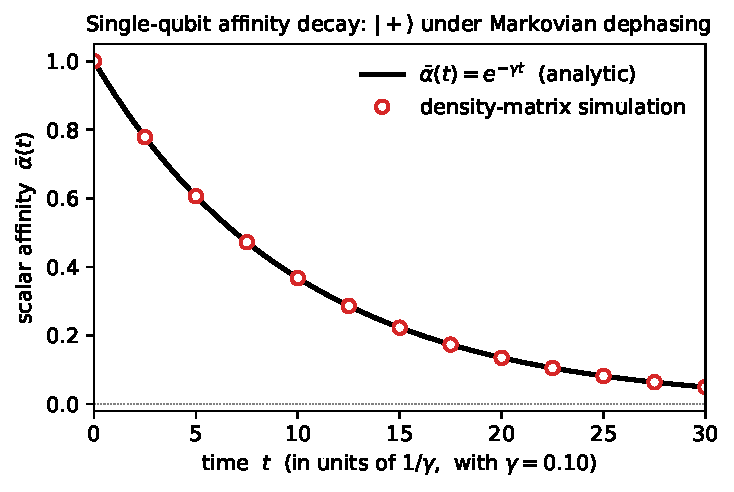
\includegraphics[width=0.85\columnwidth]{fig1_affinity_decay}
\caption{Decay of the scalar affinity $\bar{\alpha}(t)$ for a qubit
  initialized in $\vert+\rangle = (\vert\pi_0\rangle
  + \vert\pi_1\rangle)/\sqrt{2}$ under Markovian dephasing at rate
  $\gamma = 0.10$.
  The solid curve is the analytic result
  $\bar{\alpha}(t) = e^{-\gamma t}$ (Proposition~\ref{prop:determination});
  circles show values from the numerical density-matrix simulation of
  Sec.~\ref{sec:sim}.
  The dashed line marks $\bar{\alpha} = 0$, the classical limit of
  complete decoherence.}
\label{fig:affinity-decay}
\end{figure}

% ── III.D  Proposition III ───────────────────────────────────────────────────

\subsection{\label{sec:prop3}Proposition~III:
            Coherence--Affinity Correspondence}

\begin{proposition}[Coherence--Affinity Correspondence]
\label{prop:correspondence}
The scalar affinity satisfies $\bar{\alpha}(S,E) \in [0,1]$, with:
\begin{enumerate}
  \item[\emph{(i)}] $\bar{\alpha}(S,E) = 0$ if and only if $\rho_S$
    is diagonal in the pointer basis (complete decoherence);
  \item[\emph{(ii)}] $\bar{\alpha}(S,E) = 1$ if and only if $\rho_S$
    is a pure state of the form
    $\vert\psi\rangle = d^{-1/2}\sum_k e^{i\phi_k}\vert\pi_k\rangle$
    for real phases $\phi_k$ (equal-weight pointer-basis superposition);
  \item[\emph{(iii)}] $\bar{\alpha}(S,E;t)$ is continuous in $t$ and
    monotonically non-increasing under the dephasing evolution of
    Proposition~\ref{prop:determination}, strictly decreasing whenever
    $\bar{\alpha}(S,E;0) > 0$.
\end{enumerate}
\end{proposition}

\begin{proof}
\emph{Range.}
Since $\rho_S \geq 0$ and $\mathrm{Tr}[\rho_S] = 1$, the Cauchy--Schwarz
inequality gives
$\lvert\rho_{ij}\rvert^2 \leq \rho_{ii}\,\rho_{jj}$ for all $i,\,j$.
Summing over $i \neq j$:
\begin{equation*}
  \bigl\lVert\alpha\bigr\rVert_F^2
  \;=\; \sum_{i\neq j}\lvert\rho_{ij}\rvert^2
  \;\leq\; \sum_{i\neq j}\rho_{ii}\,\rho_{jj}
  \;=\; \Bigl(\sum_k\rho_{kk}\Bigr)^2 - \sum_k\rho_{kk}^2
  \;=\; 1 - \sum_k\rho_{kk}^2
  \;\leq\; \frac{d-1}{d},
\end{equation*}
where the last step uses $\sum_k\rho_{kk}^2 \geq 1/d$ by the
power-mean inequality.
Multiplying by $d/(d-1)$ and taking the square root gives
$\bar{\alpha} \leq 1$.
Non-negativity is immediate from the definition.

\emph{Part (i).}
$\bar{\alpha} = 0 \Leftrightarrow \lVert\alpha\rVert_F = 0
\Leftrightarrow \rho_{ij} = 0$ for all $i \neq j
\Leftrightarrow \rho_S$ diagonal in pointer basis.

\emph{Part (ii).}
$\bar{\alpha} = 1$ requires equality throughout the range bound.
Writing any purification of $\rho_S$ as
$\rho_S = \sum_m\vert\phi_m\rangle\langle\phi_m\vert$ with
$\lvert\rho_{ij}\rvert^2
  = \bigl\lvert\sum_m\overline{\langle\phi_m\vert\pi_i\rangle}
                       \langle\phi_m\vert\pi_j\rangle\bigr\rvert^2$,
the Cauchy--Schwarz equality
$\lvert\rho_{ij}\rvert^2 = \rho_{ii}\rho_{jj}$ holds for a single pair
$(i,j)$ iff the column vectors
$(\langle\phi_m\vert\pi_i\rangle)_m$ and
$(\langle\phi_m\vert\pi_j\rangle)_m$ are proportional;
equality at \emph{every} off-diagonal pair forces all such columns to be
proportional, hence $\mathrm{rank}\,\rho_S \leq 1$, i.e., $\rho_S$ is a
pure state.
The power-mean equality $\sum_k\rho_{kk}^2 = 1/d$ holds iff
$\rho_{kk} = 1/d$ for all $k$.
Together these require $\rho_S = \vert\psi\rangle\langle\psi\vert$
with $\lvert\langle\pi_k\vert\psi\rangle\rvert^2 = 1/d$, i.e.,
$\vert\psi\rangle = d^{-1/2}\sum_k e^{i\phi_k}\vert\pi_k\rangle$.

\emph{Part (iii).}
Continuity follows from the continuity of $\rho_{ij}(t) = \rho_{ij}(0)e^{-\gamma t}$.
Monotonicity follows from $\bar{\alpha}(t) = \bar{\alpha}(0)e^{-\gamma t}$
and $\gamma > 0$.
\end{proof}

\begin{remark}[Affinity vs.\ entanglement]
\label{rem:affinity-vs-entanglement}
A potential source of confusion merits explicit comment.
$\bar{\alpha}$ measures the quantum coherence of the \emph{local}
reduced state $\rho_S$ in the pointer basis; it is \emph{not}
a measure of bipartite entanglement between $S$ and $E$.
Indeed, $\bar{\alpha}(S,E) = 1$ corresponds to a pure superposition of
pointer states that $E$ has not yet correlated with --- in a product
initial state $\vert\psi_0\rangle_S\vert 0\rangle_E$, this is the
state of \emph{zero} $S$-$E$ entanglement.
As decoherence proceeds and $\bar{\alpha}$ decreases toward zero,
$S$-$E$ entanglement grows (see Proposition~\ref{prop:conservation}).
The two quantities are inversely related along the decoherence
trajectory, which is made precise in Proposition~\ref{prop:conservation}.
\end{remark}

% ── III.E  Proposition IV ────────────────────────────────────────────────────

\subsection{\label{sec:prop4}Proposition~IV:
            Coherence Redistribution under Unitary $S$--$E$ Evolution}

The three identities collected below are standard~--- purity
conservation under unitary evolution, the
$I(S{:}E) = 2S(\rho_S)$ identity from the Schmidt
decomposition~\cite{NielsenChuang2000}, and the Joos--Zeh / Zurek
branching identity for environment-induced
decoherence~\cite{JoosZeh1985,Zurek2003}~--- and I do not claim
novelty for them.
Their utility here is the explicit packaging in $\bar\alpha$-language,
which renders the export of local pointer-basis coherence into
$S$--$E$ correlations as a coherence-budget statement that can be
read off layer by layer in a quantum circuit.

\begin{proposition}[Coherence redistribution under unitary $S$--$E$ evolution]
\label{prop:conservation}
Let $S{+}E$ be a closed system evolving unitarily from a pure initial
product state $\rho_{SE}(0)
  = \vert\psi_0\rangle_S\vert 0\rangle_E\langle 0\vert\langle\psi_0\vert$
under a pointer-basis-coupling Hamiltonian
$H_{\mathrm{int}} = \sum_k\vert\pi_k\rangle\langle\pi_k\vert\otimes B_k$
that yields the pure-dephasing dynamics of
Proposition~\ref{prop:determination}.
Parts (i) and (iii) hold generally under this closed-system unitary
hypothesis; part (ii) additionally requires the Markovian regime, as
stated explicitly in its own itemization below.
\begin{enumerate}
  \item[\emph{(i)}] \emph{Purity conservation.}
    $\mathrm{Tr}[\rho_{SE}(t)^2] = 1$ for all $t \geq 0$.
  \item[\emph{(ii)}] \emph{Mutual information growth (Markovian regime).}
    In the Markovian pure-dephasing limit of
    Proposition~\ref{prop:determination}~--- equivalently, when the
    environmental branch overlaps
    $\lvert\langle E_j(t)\vert E_i(t)\rangle\rvert$ decay monotonically
    in $t$~--- the quantum mutual information
    $I(S\!:\!E;\,t) = 2\,S(\rho_S(t))$ is non-decreasing, where
    $S(\cdot)$ is the von Neumann entropy.
    For finite non-Markovian environments the branch overlaps can revive
    and $S(\rho_S(t))$ and $I(S\!:\!E;\,t)$ can decrease (information
    backflow); the assertion does not extend to that regime.
  \item[\emph{(iii)}] \emph{Coherence transfer.}
    Writing $\vert\psi(t)\rangle = \sum_k c_k\,
    \vert\pi_k\rangle\vert E_k(t)\rangle$ with
    $c_k = \langle\pi_k\vert\psi_0\rangle$,
    \begin{equation}
    \label{eq:coherence-transfer}
      \langle\pi_i\vert\rho_S(t)\vert\pi_j\rangle
      \;=\; c_i\,c_j^*\;\langle E_j(t)\vert E_i(t)\rangle,
      \qquad i \neq j,
    \end{equation}
    so that $\bar{\alpha}(t) \to 0$ if and only if
    $\langle E_j(t)\vert E_i(t)\rangle \to 0$ for every pair $i \neq j$
    with $c_i c_j^* \neq 0$ (off-diagonals at populations $c_i = 0$
    or $c_j = 0$ vanish trivially).
\end{enumerate}
\end{proposition}

\begin{proof}
\emph{Part (i).}
Unitary evolution $\rho_{SE}(t) = U(t)\rho_{SE}(0)U^\dagger(t)$
preserves the spectrum of $\rho_{SE}$, hence its purity
$\mathrm{Tr}[\rho_{SE}^2]$.
Since $\rho_{SE}(0)$ is rank-one, $\mathrm{Tr}[\rho_{SE}(0)^2] = 1$,
and the result follows.

\emph{Part (ii).}
For a pure bipartite state $\rho_{SE}$, the Schmidt decomposition
gives $S(\rho_S) = S(\rho_E)$ and $S(\rho_{SE}) = 0$, hence
$I(S\!:\!E) = S(\rho_S) + S(\rho_E) - S(\rho_{SE}) = 2\,S(\rho_S)$.
In the Markovian regime of
Proposition~\ref{prop:determination}~--- equivalently, monotonic
decay of $\lvert\langle E_j(t)\vert E_i(t)\rangle\rvert$~--- the induced
channel on $\rho_S$ between any two times $t_1 < t_2$ preserves
diagonal populations in the pointer basis [part~(iii) below; in the
Markovian limit, $\sum_k L_k^\dagger L_k = \gamma\,\mathbf{I}$], is
CP-divisible, and is therefore unital: it preserves the maximally
mixed state.
Unital channels mix the spectrum in the majorization order,
$\lambda(\rho_S(t_2)) \prec \lambda(\rho_S(t_1))$~\cite{NielsenChuang2000}.
Since von Neumann entropy is Schur-concave, $S(\rho_S(t))$ is
non-decreasing in $t$, and consequently so is $I(S\!:\!E;\,t)$.
For non-Markovian dynamics the induced channel between $t_1$ and $t_2$
need not be CP-divisible, the unital-channel argument fails, and
$S(\rho_S(t))$ can decrease whenever the environmental branch overlaps
revive; the standard physical signature is information backflow into
$S$.

\emph{Part (iii).}
A pointer-basis interaction
$H_{\mathrm{int}} = \sum_k\vert\pi_k\rangle\langle\pi_k\vert\otimes B_k$
acting on the product initial state generates conditional environmental
branches $\vert E_k(t)\rangle = e^{-iB_k t/\hbar}\vert 0\rangle_E$
(generally not orthonormal), so the joint state takes the form
$\vert\psi(t)\rangle = \sum_k c_k\,\vert\pi_k\rangle\vert E_k(t)\rangle$
with $c_k = \langle\pi_k\vert\psi_0\rangle$.
The reduced density matrix is
\begin{equation*}
  \rho_S(t) = \mathrm{Tr}_E\!\bigl[\vert\psi(t)\rangle\langle\psi(t)\vert\bigr]
  = \sum_{i,j} c_i c_j^*\,\langle E_j(t)\vert E_i(t)\rangle\,
    \vert\pi_i\rangle\langle\pi_j\vert,
\end{equation*}
from which Eq.~\eqref{eq:coherence-transfer} follows directly.
For each $i\neq j$ with $c_i c_j^* \neq 0$, the off-diagonal magnitude
$\lvert\rho_{ij}(t)\rvert = \lvert c_i c_j^*\rvert\,
\lvert\langle E_j(t)\vert E_i(t)\rangle\rvert$ is monotonically tied to
the environmental overlap; the Markovian approximation leading to
Eq.~\eqref{eq:alpha-decay} corresponds to
$\lvert\langle E_j(t)\vert E_i(t)\rangle\rvert = e^{-\gamma t}$.
When $\langle E_j(t)\vert E_i(t)\rangle = 0$ for every $i\neq j$ with
$c_i c_j^* \neq 0$, the populated branches form an orthonormal set and
$S$ has acquired a definite pointer-state record in $E$: no coherence
has been destroyed --- it has been redistributed into the
distinguishability of $\{\vert E_k\rangle\}$.
\end{proof}

\begin{remark}[Coherence as a circuit-level resource]
Proposition~\ref{prop:conservation} has a direct bearing on the
design of the $\URA$ gate (Sec.~\ref{sec:gate}).
Because decoherence transfers, rather than destroys, relational
structure, the local pointer-basis coherence
$\bar{\alpha}(t) = \bar{\alpha}(0)\,e^{-\gamma t}$ available at time $t$
is a finite, monotonically depleting budget.
A two-qubit entangling operation expends a portion of this budget per
gate by redistributing local coherence into $S$-$E$ correlations
[Eq.~\eqref{eq:coherence-transfer}]; an operation acting below its
maximum entanglement capability expends a smaller portion, leaving more
coherence available for downstream layers.
The conservation law also sets a hard upper bound: no unitary acting on
$S$ alone (without access to $E$) can increase $\bar{\alpha}(t)$ above
its current value, so the coherence-preservation strategy is to
\emph{spend less per gate}, not to attempt local recovery.
This is the operational content the $\URA(\theta)$ gate of
Sec.~\ref{sec:gate} exploits.
\end{remark}

% ── SECTION 4: TUNABLE ISOTROPIC-EXCHANGE GATE (~1,100 words) ────────────────

\section{The Tunable Isotropic-Exchange Gate in the \RCF{} Diagnostic}
\label{sec:gate}

\subsection{Definition}

The \RCF~packages the dynamics of pointer-basis coherence as a
continuous resource: the scalar affinity $\bar\alpha(S,E)$ ranges over
$[0,1]$ (Proposition~\ref{prop:correspondence}), decays continuously
under decoherence (Proposition~\ref{prop:determination}), and is
redistributed into $S$--$E$ correlations rather than destroyed
under unitary $S$--$E$ evolution (Proposition~\ref{prop:conservation}).
The corresponding hardware engineering picture~--- that the natural
two-qubit primitive should expose a continuous coupling angle, tunable
to the coherence budget of the substrate rather than fixed to a
particular entanglement capability~--- is by now well established.
Continuously parameterized two-qubit exchange gates are realized as
the native primitive on Loss--DiVincenzo spin
qubits~\cite{LossDiVincenzo1998}, as parametric entangling gates on
transmon platforms~\cite{Caldwell2018}, and as the continuous fSim/$XY$
families demonstrated on Sycamore-class
hardware~\cite{Foxen2020,Abrams2020,Lacroix2020}.
The contribution of the present section is not the unitary itself~--- it
is the standard isotropic Heisenberg-exchange family~--- but the
coherence-budget framing of its parameter selection through the
$\bar\alpha$-language of Sec.~\ref{sec:rct}.

\begin{definition}[Tunable isotropic-exchange gate]
\label{def:ura}
I denote by
\begin{equation}
  \URA(\theta) = \exp\!\left(-\frac{i\theta}{2}
    \bigl(\sigma_x \otimes \sigma_x
         + \sigma_y \otimes \sigma_y
         + \sigma_z \otimes \sigma_z\bigr)\right),
  \label{eq:URA}
\end{equation}
the two-qubit unitary on the isotropic Heisenberg-exchange axis,
where $\theta \in [0, \pi/2]$ is the \emph{exchange angle}~--- the
Hamiltonian evolution parameter (coupling$\,\times\,$time) along this
axis~--- and $\sigma_{x,y,z}$ are the Pauli matrices acting on
$\mathbb{C}^2$.
Within the \RCF{} coherence-budget diagnostic of Sec.~\ref{sec:rct} I
refer to this use of the isotropic-exchange family as the
\emph{relational-affinity parameterization}; the unitary itself is the
standard exchange family and is not a new gate.
\end{definition}

The operator $G \equiv \sigma_x\otimes\sigma_x +
\sigma_y\otimes\sigma_y + \sigma_z\otimes\sigma_z$ appearing inside
the exponent of Eq.~\eqref{eq:URA} is, up to an overall factor of
$1/2$, the isotropic Heisenberg exchange interaction, established by
Loss and DiVincenzo~\cite{LossDiVincenzo1998} as a universal two-qubit
primitive for solid-state quantum computation and the natural exchange
coupling realized on a range of superconducting and spin-qubit
platforms~\cite{Krantz2019,Caldwell2018,Foxen2020,Abrams2020};
$G$ generates entanglement symmetrically across all three Pauli axes.
The exchange angle~$\theta$ controls the magnitude of relational coupling
effectuated between the two qubits in a single operation; its connection
to the scalar affinity $\bar\alpha$ of Sec.~\ref{sec:rct} is
\emph{indirect}, and I make the relationship explicit here to forestall
a natural confusion.
$\bar\alpha(S,E)$ measures the local pointer-basis coherence remaining in
the reduced state $\rho_S$ (Definition~\ref{def:alpha-scalar}), whereas
$\theta$ parameterizes the coupling strength of a unitary applied to a
two-qubit system; the two have different domains
($\bar\alpha \in [0,1]$ versus $\theta \in [0,\pi/2]$) and respond
inversely along a decoherence trajectory: as $\theta$ increases toward
$\pi/4$, the gate generates more $S$-$S'$ entanglement, and the
post-gate marginal $\rho_S$ moves toward the maximally mixed state with
$\bar\alpha \to 0$ (cf.\ Proposition~\ref{prop:conservation}, part~(iii)
and the Affinity-vs.-Entanglement remark in Sec.~\ref{sec:prop3}).
What the \RCF~contributes is the conceptual warrant for a continuously
parameterized exchange gate~--- namely, that relational coupling is
itself continuous and conservatively redistributed~--- not a
quantitative identity $\theta = \bar\alpha$.

In the computational basis $\{\ket{00}, \ket{01}, \ket{10}, \ket{11}\}$,
the gate takes the explicit form
\begin{equation}
  \URA(\theta) =
  \begin{pmatrix}
    e^{-i\theta/2} & 0 & 0 & 0 \\
    0 & e^{i\theta/2}\cos\theta & {-i}\,e^{i\theta/2}\sin\theta & 0 \\
    0 & {-i}\,e^{i\theta/2}\sin\theta & e^{i\theta/2}\cos\theta & 0 \\
    0 & 0 & 0 & e^{-i\theta/2}
  \end{pmatrix}.
  \label{eq:URA-matrix}
\end{equation}
This form follows from the spectral decomposition of the generator $G =
\sigma_x\!\otimes\!\sigma_x + \sigma_y\!\otimes\!\sigma_y + \sigma_z\!\otimes\!\sigma_z$,
whose eigenvalues are $+1$ (triplet, three-fold: $\ket{00}$, $\ket{11}$,
$\ket{\Psi^+}$) and $-3$ (singlet: $\ket{\Psi^-}$).
Accordingly, $\URA(\theta)$ acts on the two invariant subspaces independently:
the triplet states $\ket{00}$ and $\ket{11}$ each acquire the phase $e^{-i\theta/2}$,
while states in the $\{\ket{01},\ket{10}\}$ subspace receive a mixture of
the triplet phase $e^{-i\theta/2}$ and singlet phase $e^{3i\theta/2}$,
producing the coherent rotation seen in the central $2\times2$ block.
At $\theta = 0$, $\URA = \mathbf{I}_4$ (identity).
At $\theta = \pi/4$, the gate achieves maximum entanglement capability
(see Section~\ref{subsec:weyl}).
At $\theta = \pi/2$, $\URA$ reduces to the \textsc{swap} gate up to
local operations.

\subsection{Bell State Production}
\label{subsec:bell}

The gate's entangling action is most directly illustrated by its
behaviour on the computational basis state $\ket{01}$ at $\theta = \pi/4$.
Because $\ket{01} = \tfrac{1}{\sqrt{2}}(\ket{\Psi^+} + \ket{\Psi^-})$
decomposes into equal triplet ($\ket{\Psi^+}$, eigenvalue $+1$) and
singlet ($\ket{\Psi^-}$, eigenvalue $-3$) components of the generator $G$,
the gate applies distinct phase factors to each branch.
Reading from Eq.~\eqref{eq:URA-matrix}:
\begin{equation}
  \URA(\pi/4)\ket{01}
    = \frac{e^{i\pi/8}}{\sqrt{2}}\bigl(\ket{01} - i\ket{10}\bigr),
  \label{eq:bell-production}
\end{equation}
a maximally entangled state with concurrence $\mathcal{C} = 1$,
consistent with the entanglement capability peak at $\theta = \pi/4$
(Sec.~\ref{subsec:entcap}).
The global phase $e^{i\pi/8}$ is physically unobservable.

States lying entirely within the triplet sector~--- $\ket{00}$, $\ket{11}$,
and $\ket{\Psi^+}$~--- each acquire only the phase $e^{-i\theta/2}$ under
$\URA(\theta)$ and remain unentangled.
Entanglement generation therefore requires an input state with nonzero
singlet weight $\langle\Psi^-\vert\psi_{\rm in}\rangle \neq 0$.
All four Bell states are accessible from the computational basis via
$\URA(\pi/4)$ composed with appropriate single-qubit Pauli corrections,
confirming that $\URA$ spans the full entanglement capability of the
two-qubit Hilbert space.

\subsection{Weyl Chamber Analysis}
\label{subsec:weyl}

Two-qubit gates are classified up to local operations by their position in
the Weyl chamber of $\mathrm{SU}(4)/[\mathrm{SU}(2)\otimes\mathrm{SU}(2)]$,
parameterized by coordinates $(c_1, c_2, c_3) \in [0,\pi/2]^3$ with
$c_1 \geq c_2 \geq c_3 \geq 0$~\cite{Zhang2003WeylChamber}.
These coordinates are extracted from the \emph{local invariants} of the
two-qubit gate matrix and correspond to the canonical Cartan
decomposition $A = \exp\!\bigl[i(c_1\,\sigma_x{\otimes}\sigma_x +
c_2\,\sigma_y{\otimes}\sigma_y + c_3\,\sigma_z{\otimes}\sigma_z)/2\bigr]$
in the standard convention of Zhang et al., in which \textsc{swap}
sits at $(\pi/2, \pi/2, \pi/2)$.

For $\URA(\theta)$, the Weyl chamber coordinates are:
\begin{equation}
  c_1(\theta) = \theta, \qquad
  c_2(\theta) = \theta, \qquad
  c_3(\theta) = \theta.
  \label{eq:weyl-coords}
\end{equation}
The trajectory $(c_1, c_2, c_3) = (\theta, \theta, \theta)$ lies along the
main diagonal of the Weyl chamber, tracing the \emph{Heisenberg family} from the
identity ($\theta = 0$, corner $O$) to the \textsc{swap} point ($\theta = \pi/2$).
The maximally entangling point $\theta = \pi/4$ sits at Weyl coordinates
$(\pi/4, \pi/4, \pi/4)$~--- the interior midpoint of this diagonal~--- and is
not locally equivalent to any of the standard fixed gates.

This trajectory is significant: fixed standard gates occupy single
\emph{points} in the Weyl chamber~--- \textsc{cnot} at $(\pi/2, 0, 0)$,
\textsc{iswap} at $(\pi/2, \pi/2, 0)$, \textsc{cz} at $(\pi/2, 0, 0)$
(locally equivalent to \textsc{cnot}).
The gate $\URA(\theta)$ instead traces a \emph{continuous path} parameterized
by~$\theta$, covering a range of entanglement capabilities rather than a
single fixed point.

\subsection{Entanglement Capability}
\label{subsec:entcap}

The \emph{entanglement capability} $\mathcal{E}(\theta)$ of a two-qubit gate
is the maximum concurrence achievable over all product input
states~\cite{Zhang2003WeylChamber}:
\begin{equation}
  \mathcal{E}(\theta) = \max_{\ket{\phi_1}\otimes\ket{\phi_2}}
    \mathcal{C}\!\left(\URA(\theta)\ket{\phi_1\phi_2}\right).
  \label{eq:entcap}
\end{equation}
For $\URA(\theta)$ with Weyl coordinates $(\theta, \theta, \theta)$,
the entanglement capability is:
\begin{equation}
  \mathcal{E}(\theta) = |\sin(2\theta)|,
  \label{eq:entcap-result}
\end{equation}
which rises monotonically on $[0, \pi/4]$ from
$\mathcal{E}(0) = 0$ to the maximum $\mathcal{E}(\pi/4) = 1$
(the $\sqrt{\textsc{swap}}$ point) and decreases symmetrically on
$[\pi/4, \pi/2]$ back to $\mathcal{E}(\pi/2) = 0$ (the \textsc{swap}
gate, which permutes states without generating entanglement).

The practical implication is direct: by selecting $\theta < \pi/4$ on
hardware whose decoherence rate is non-negligible and whose
two-qubit-gate duration scales linearly with the exchange angle, the
gate trades a fraction of its entanglement capability for a
proportionally shorter operation time, accumulating less coherence-limited
noise per gate (Sec.~\ref{sec:sim}, Eq.~\eqref{eq:peff}).
Combined with the gate-time-proportional noise model of
Sec.~\ref{sec:sim} [Eq.~\eqref{eq:peff}], the coherence redistribution
structure of Proposition~\ref{prop:conservation} renders the per-gate
$\bar\alpha$ cost of a partial-exchange operation as a strictly smaller
fraction than that of a full maximally-entangling operation: Proposition~\ref{prop:conservation} supplies the redistribution
identity, and the gate-time scaling supplies the proportionality.
The fixed-angle gates \textsc{cnot}, \textsc{iswap}, and \textsc{cz}
occupy single points of the Weyl chamber and do not admit this
trade-off without explicit compilation; the continuous fSim/$XY$ and
parametric exchange families~\cite{Foxen2020,Abrams2020,Lacroix2020,Caldwell2018}
are analogous hardware-native tunable primitives.
In Weyl-chamber language the fSim family traces
$(c_1,c_2,c_3) = (\theta,\theta,\varphi)$ with independent iSWAP-like
$\theta$ and CZ-like $\varphi$, of which $\URA(\theta)$ is the isotropic
specialization $\varphi = \theta$.
On Sycamore-class hardware
Foxen~\textit{et~al.}\ have demonstrated experimentally the fidelity
advantage of operating at a continuously-tunable, fractional-exchange
parameter relative to a fixed entangler.
Sec.~\ref{sec:sim} quantifies the corresponding advantage of
$\URA(\theta < \pi/4)$ in independent simulation, with explicit caveats
on the scope of applicability in Sec.~\ref{sec:disc}.

% ── SECTION 5: NUMERICAL SIMULATION RESULTS (~1,500 words) ──────────────────

\section{Numerical Simulation}
\label{sec:sim}

\subsection{Implementation}

I implement $\URA(\theta)$ as a two-qubit unitary operator via the
explicit matrix form of Eq.~\eqref{eq:URA-matrix} in both
Qiskit~\cite{Qiskit2024} (IBM) and Cirq~\cite{Cirq2025} (Google).
Simulation parameters follow Appendix~\ref{app:sim-params}.
The circuit representation is:

\begin{center}
\begin{quantikz}
  \lstick{$\ket{0}$} & \gate[2]{U_{\mathrm{RA}}(\theta)} & \qw \\
  \lstick{$\ket{0}$} &                                    & \qw
\end{quantikz}
\end{center}

\noindent
Performance is benchmarked against three fixed two-qubit gates~--- \textsc{cnot},
\textsc{iswap}, and \textsc{cz}~--- which are the standard entangling
primitives on IBM and Google hardware respectively.
The key distinction is that these fixed gates always operate at full
entanglement capability ($\mathcal{E} = 1$), whereas $\URA(\theta)$
operates at $\mathcal{E}(\theta) = |\sin 2\theta|$
(Eq.~\eqref{eq:entcap-result}), continuously tunable via the exchange
angle.

\subsection{Noise Models and Gate-Time Scaling}

Three noise channels~\cite{NielsenChuang2000} model the dominant
decoherence mechanisms in near-term superconducting qubit devices:

\begin{enumerate}
  \item \textbf{Depolarizing noise:}
    $\mathcal{E}(\rho) = (1-p)\rho + \tfrac{p}{4}\mathbf{I}_4$,
    where $p \in [0.01, 0.10]$ is the per-gate error rate.
  \item \textbf{Dephasing (phase damping):}
    $\rho_{ij} \mapsto \rho_{ij}(1-\gamma)^{d_{ij}}$,
    where $d_{ij}$ is the Hamming distance between bitstrings $i$ and $j$
    and $\gamma \in [0.02, 0.20]$.
  \item \textbf{Amplitude damping:}
    Kraus channel with $T_1$ relaxation probability
    $p_{\mathrm{AD}} \in [0.02, 0.20]$, applied independently to each qubit.
\end{enumerate}

A critical physical consideration governs the comparison.
On hardware where the two-qubit-gate pulse duration is set by the
Heisenberg exchange coupling and the gate is directly calibrated as a
single continuous parameter~--- spin-qubit exchange platforms, certain
parametric transmon architectures, and Sycamore-class tunable
couplers~\cite{LossDiVincenzo1998,Caldwell2018,Foxen2020,Abrams2020}~--- the
coherence-limited contribution to two-qubit gate error accumulates in
proportion to gate duration~\cite{Krantz2019}, and the
exchange-angle pulse duration scales linearly with~$\theta$: running at
$\theta = \pi/8$ takes half the time of a full $\theta = \pi/4$
($\sqrt{\textsc{swap}}$) operation.
I therefore postulate \emph{gate-time-proportional noise}: fixed gates
(\textsc{cnot}, \textsc{iswap}, \textsc{cz}) receive error rate~$p_{\rm base}$
at full duration, while $\URA(\theta)$ receives effective rate
\begin{equation}
  p_{\rm eff}(\theta) = p_{\rm base} \times \frac{\theta}{\pi/4},
  \label{eq:peff}
\end{equation}
reflecting shorter physical operation time for $\theta < \pi/4$.
Equation~\eqref{eq:peff} encodes the small-$p$, leading-order
linearization in which each channel's per-gate error contribution is
proportional to physical pulse duration; saturating corrections
(e.g., the $1 - e^{-t/T_1}$ form of amplitude damping at large
$t/T_1$) are negligible to the order reported in
Table~\ref{tab:fidelity-all}.
This is a modelling assumption appropriate to coherence-limited error on
direct-exchange hardware; it does not capture coherent calibration
error, leakage to non-computational levels, or spectator-qubit
crosstalk, all of which can have different scalings with~$\theta$.
On platforms where $\URA(\theta)$ must be decomposed into fixed native
primitives, the advantage below depends on the decomposition cost and
may shrink or vanish (cf.\ Sec.~\ref{sec:disc}).

\subsection{Results}

\textbf{Gate fidelity advantage.}
Table~\ref{tab:fidelity} reports the average gate
fidelity~\cite{Nielsen2002Fidelity}
\begin{equation}
  F_{\rm avg}(W, V) \;=\; \frac{d\,F_{\rm proc}(W, V) + 1}{d + 1},
  \qquad
  F_{\rm proc}(W, V) \;=\; \mathrm{Tr}[\chi_V^\dagger\,\chi_W],
  \label{eq:favg}
\end{equation}
of each gate under depolarizing noise with gate-time-proportional
error scaling, where $d = 4$ for two qubits and $\chi_V$, $\chi_W$ are
the Choi--Jamio\l{}kowski process matrices of the ideal and noisy
implementations respectively.
For the global depolarizing channel $W(\rho) = (1-p_{\rm eff})\rho +
p_{\rm eff}\,\mathbf{I}_4/4$ applied after an ideal unitary, this
reduces to the closed-form expression
$F_{\rm avg} = 1 - 3\,p_{\rm eff}/4$.
The values in Table~\ref{tab:fidelity} are this analytical expression
evaluated at the gate-specific $p_{\rm eff}$ of
Eq.~\eqref{eq:peff}~--- i.e., the depolarizing column is closed-form
rather than simulator-derived.
The script \texttt{figures/\allowbreak generate\_\allowbreak tables.py} computes these values
directly from the formula, and the Qiskit/Cirq density-matrix
simulator notebooks of the release tag (Sec.~\ref{sec:conc}) reproduce
them to numerical precision under the same channel.
$\URA(\pi/4)$ (full duration, $\theta = \pi/4$) operates at maximum
entanglement capability ($\mathcal{E} = 1$).
Under the global depolarizing channel~--- which is unitary-invariant~--- the
average gate fidelity depends only on $p_{\rm eff}$, so $\URA(\pi/4)$ and
\textsc{iswap} achieve identical $F_{\rm avg}$ at equal duration; the
partial-exchange advantage I report below is therefore at $\theta < \pi/4$.
$\URA(\pi/8)$ (half duration, $\theta = \pi/8$) achieves measurable
advantages: $\Delta F = +0.019$ at $p_{\rm base} = 0.05$ and $+0.038$ at
$p_{\rm base} = 0.10$ over all three fixed gates under depolarizing noise.

\begin{table}[htbp]
\centering
\caption{Average gate fidelity under depolarizing noise (gate-time-proportional
model). Values are the closed-form expression
$F_{\rm avg} = 1 - 3 p_{\rm eff}/4$ evaluated at the gate-specific
$p_{\rm eff}$ of Eq.~\eqref{eq:peff}; the Qiskit/Cirq simulator
notebooks of the release tag reproduce these values to numerical
precision. $p_{\rm base}$ = error rate per full-duration two-qubit
gate. $\URA(\pi/8)$ operates at $0.50\times$ gate duration;
$\URA(\pi/6)$ at $0.67\times$.}
\label{tab:fidelity}
\begin{tabular}{lccccl}
\toprule
Gate & $p=0.01$ & $p=0.02$ & $p=0.05$ & $p=0.10$ & Duration \\
\midrule
\textsc{cnot}    & 0.9925 & 0.9850 & 0.9625 & 0.9250 & $1.00\times$ \\
\textsc{iswap}   & 0.9925 & 0.9850 & 0.9625 & 0.9250 & $1.00\times$ \\
\textsc{cz}      & 0.9925 & 0.9850 & 0.9625 & 0.9250 & $1.00\times$ \\
\midrule
$\URA(\pi/4)$    & 0.9925 & 0.9850 & 0.9625 & 0.9250 & $1.00\times$ \\
$\URA(\pi/6)$    & 0.9950 & 0.9900 & 0.9750 & 0.9500 & $0.67\times$ \\
$\URA(\pi/8)$    & \textbf{0.9962} & \textbf{0.9925} & \textbf{0.9812} & \textbf{0.9625} & $0.50\times$ \\
\bottomrule
\end{tabular}
\end{table}

\textbf{Consistency across noise models.}
Table~\ref{tab:fidelity-all} reports the fidelity advantage
$\Delta F = F[\URA(\pi/8)] - F[\textsc{iswap}]$ at $p_{\rm base} \in \{0.02, 0.05, 0.10\}$
across all three noise models.
The depolarizing row is the closed-form value
$\Delta F = 3\,p_{\rm base}/8$ obtained from $F_{\rm avg} = 1 - 3 p_{\rm eff}/4$
with $p_{\rm eff}(\URA(\pi/8)) = p_{\rm base}/2$ and
$p_{\rm eff}(\textsc{iswap}) = p_{\rm base}$ [Eq.~\eqref{eq:peff}].
The dephasing and amplitude-damping rows are obtained by
density-matrix simulation in Qiskit and Cirq with per-qubit Kraus
channels applied as a post-gate composition at the
gate-time-scaled rate (see App.~\ref{app:sim-params} for the explicit
Kraus operators and the application point).
I emphasize that the near-equality between the depolarizing,
dephasing, and amplitude-damping rows is not a coincidence: under
gate-time-proportional, small-$p$, post-gate channels the leading-order
contribution to $1 - F_{\rm avg}$ is linear in the per-qubit error rate
and identical across the three channels up to channel-specific
constants of order unity, with the closed-form depolarizing value
$\Delta F = 3\,p_{\rm base}/8$ serving as a tight reference
(Table~\ref{tab:fidelity-all} caption).
With that interpretation in mind, the simulations confirm that the
gate-time-saving translates to a per-gate fidelity advantage of
$\Delta F \in [+0.038, +0.039]$ at $p_{\rm base} = 0.10$ across all
three channels and $\Delta F \in [+0.019, +0.020]$ at
$p_{\rm base} = 0.05$.

\begin{table}[htbp]
\centering
\caption{Fidelity advantage $\Delta F = F[\URA(\pi/8)] - F[\mathrm{iSWAP}]$
under gate-time-proportional noise. Depolarizing row: closed-form
analytical values ($\Delta F = 3 p_{\rm base}/8$). Dephasing
(per-qubit Pauli-$Z$ with off-diagonal damping $1{-}\gamma$ per qubit,
equivalent to $p_Z = \gamma/2$) and amplitude-damping (per-qubit
standard Kraus) rows: Qiskit and Cirq density-matrix simulations agree
to numerical precision and are reproduced by the analytical formulas
in \texttt{figures/\allowbreak generate\_\allowbreak tables.py}. Positive values confirm that
$\URA(\pi/8)$ outperforms the fixed gates in all noise regimes tested.
The near-equality across rows is not a discovery of cross-channel
robustness; it is a quantitative consequence of the gate-time scaling
of Eq.~\eqref{eq:peff} in the small-noise regime (see discussion
below).}
\label{tab:fidelity-all}
\begin{tabular}{lccc}
\toprule
Noise model & $p_{\rm base} = 0.02$ & $p_{\rm base} = 0.05$ & $p_{\rm base} = 0.10$ \\
\midrule
Depolarizing    & $+0.0075$ & $+0.0187$ & $+0.0375$ \\
Dephasing       & $+0.0079$ & $+0.0196$ & $+0.0385$ \\
Amplitude damp. & $+0.0080$ & $+0.0198$ & $+0.0393$ \\
\bottomrule
\end{tabular}
\end{table}

\textbf{Interpretation via the \RCF.}
The fidelity advantage is naturally read off in the
$\bar\alpha$-language of Proposition~\ref{prop:conservation}.
A gate operating at $\theta < \pi/4$ implements a weaker exchange
interaction and consequently requires less physical interaction time
with the bath, accumulating less decoherence per operation.
Operationally, this means a smaller fraction of the local pointer-basis
coherence budget $\bar\alpha$ (Definition~\ref{def:alpha-scalar}) is
expended into $S$-bath correlations during the gate, leaving more
coherence available for downstream layers~--- exactly the redistribution
quantified by Eq.~\eqref{eq:coherence-transfer}.
For circuits requiring partial entanglement, or in which entanglement
is built incrementally across layers, $\URA(\theta)$ can therefore be
tuned to the coherence regime of the device: small $\theta$ in
high-noise environments preserves coherence that a fixed maximally
entangling gate would dissipate.
These numerics confirm the predicted gate-time scaling of the
partial-exchange family in the $\bar\alpha$-language of
Sec.~\ref{sec:rct}.

\textbf{$\bar\alpha(t)$ dynamics.}
Figure~\ref{fig:alpha-dynamics} shows the decay of $\bar\alpha(t)$ for a
two-qubit system $S$ under independent per-qubit dephasing at
$\gamma = 0.10$, initialized in the equal-weight pointer-basis
superposition
$\ket{++} = \tfrac{1}{2}(\ket{00}+\ket{01}+\ket{10}+\ket{11})$, for
which $\bar\alpha(0) = 1$ in the four-dimensional computational pointer
basis (Proposition~\ref{prop:correspondence}\emph{(ii)}).
The Affinity Operator decays monotonically from $1$ to $0$, tracking the
loss of local pointer-basis coherence as the bath selects the classical
pointer basis.
The Markovian simulation reported here traces out the bath and follows
the marginal $\rho_S$ only; in the closed unitary $S$+bath picture of
Proposition~\ref{prop:conservation}, this loss of marginal coherence
corresponds not to annihilation but to redistribution into $S$-bath
correlations, with the joint state remaining pure throughout
($\mathrm{Tr}[\rho_{S\text{-bath}}^2] = 1$).

\begin{figure}[htbp]
  \centering
  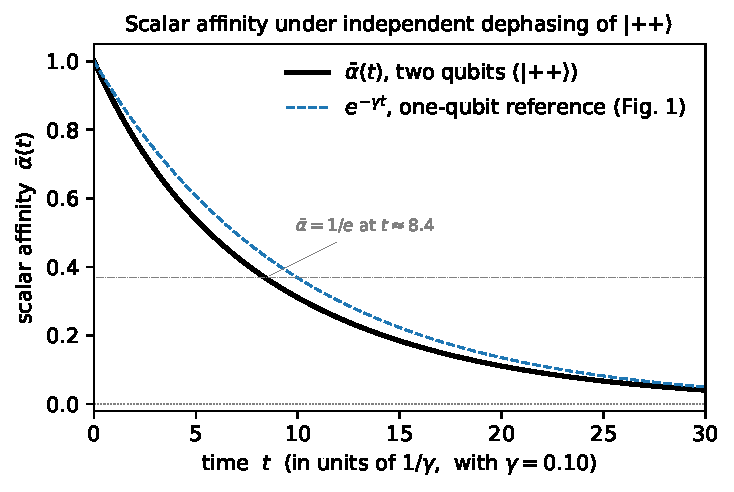
\includegraphics[width=0.85\columnwidth]{alpha-dynamics}
  \caption{Affinity Operator dynamics $\bar\alpha(t)$ for the two-qubit
    initial state $\ket{++}$ under independent per-qubit dephasing
    ($\gamma = 0.10$). The monotonic decay from $\bar\alpha = 1$ (maximal
    local pointer-basis coherence) to $\bar\alpha = 0$ (pointer-basis
    diagonal $\rho_S$) tracks the quantum-to-classical transition for
    the local state. The closed-form curve
    $\bar\alpha(t) = \sqrt{\tfrac{2}{3}e^{-2\gamma t}
                           + \tfrac{1}{3}e^{-4\gamma t}}$ reflects the
    two off-diagonal classes (Hamming distance $1$ and $2$) decaying at
    distinct rates; the dashed reference $e^{-\gamma t}$ is the
    single-qubit decay law of Fig.~\ref{fig:affinity-decay}. Total
    purity of the closed $S$+bath system is conserved throughout
    (Proposition~\ref{prop:conservation}); coherence is redistributed
    into $S$-bath correlations rather than annihilated. $\bar\alpha$
    measures local pointer-basis coherence in the reduced state of the
    full two-qubit system $\rho_S$, not $S$-bath entanglement;
    initializing instead in a Bell state $\ket{\Phi^+}_{q_1q_2}$
    (single-qubit marginals $= \mathbf{I}/2$, intra-$S$ entanglement
    maximal) yields $\bar\alpha(0) = \sqrt{2/3}$ in the four-dimensional
    computational pointer basis, not $1$.
    Generated by \texttt{figures/\allowbreak generate\_\allowbreak fig2.py}.}
  \label{fig:alpha-dynamics}
\end{figure}

% ── SECTION: COHERENCE-BUDGET ALLOCATION (~v1.0 new content) ────────────────
%   v1.0 contribution: the allocation theorem, scheduling algorithm,
%   and multi-layer fidelity benchmark.

\section{Coherence-Budget Allocation for Tunable Exchange Schedules}
\label{sec:alloc}

The per-gate fidelity comparison of Sec.~\ref{sec:sim} establishes
that, on hardware with directly calibratable Heisenberg exchange,
$\URA(\theta)$ at $\theta < \pi/4$ accumulates less coherence-limited
error than a full maximally entangling primitive at equal entangling
capability requirement.
That observation, however, says nothing about how to \emph{allocate}
entanglement across the gate layers of a circuit whose total
entanglement target is fixed.
This section turns the per-gate fidelity statement into a layerwise
optimization: given a coherence budget and an entanglement target,
how should a noise-aware compiler distribute exchange angles across
the circuit?

\subsection{Relational Coherence Cost}
\label{subsec:cost}

I define the per-layer cost of a tunable exchange gate
$\URA(\theta_\ell)$ as the local pointer-basis coherence consumed by
the gate:
%
\begin{equation}
\label{eq:layer-cost}
C_{\RCF}^{(\ell)} \;\equiv\; \bar\alpha_\ell^{\rm pre} - \bar\alpha_\ell^{\rm post}
\;=\; \bar\alpha_\ell^{\rm pre}\bigl(1 - e^{-\gamma_\ell \kappa\, \theta_\ell}\bigr),
\end{equation}
%
where $\gamma_\ell$ is the local pointer-basis dephasing rate active
during layer $\ell$ (which may vary across layers due to hardware
heterogeneity), $t_\ell = \kappa\, \theta_\ell$ is the exchange-pulse
duration on the substrate~\cite{Krantz2019}, and the exponential
form follows from
Proposition~\ref{prop:determination} in its uniform-rate Markovian
regime.
The total circuit cost is
%
\begin{equation}
\label{eq:circuit-cost}
C_{\RCF}(\mathcal{U}) \;=\; \sum_{\ell=1}^{L} C_{\RCF}^{(\ell)}.
\end{equation}
%
To leading order in $\gamma_\ell \kappa\, \theta_\ell \ll 1$
(the small-cost regime in which Eq.~\eqref{eq:peff}'s
gate-time-proportional model itself is justified, Sec.~\ref{sec:sim}),
%
\begin{equation}
\label{eq:linear-cost}
C_{\RCF}(\mathcal{U}) \;\approx\;
  \sum_{\ell=1}^{L} \tilde\gamma_\ell\, \theta_\ell,
  \qquad \tilde\gamma_\ell \equiv \bar\alpha_\ell^{\rm pre}\, \gamma_\ell\, \kappa.
\end{equation}
%
The effective rate $\tilde\gamma_\ell$ folds the substrate's exchange
time-constant and the layer's residual pre-gate coherence into a
single per-layer cost coefficient.

\subsection{Proposition~V: Exchange-Angle Coherence Cost}
\label{subsec:prop5}

The cost per layer admits a sharp closed form for the
directly-calibrated exchange-gate case treated throughout this paper.

\begin{proposition}[Exchange-angle coherence cost, Markovian regime]
\label{prop:exchange-cost}
Under uniform Markovian pointer-basis dephasing at rate $\gamma$ and the
direct exchange-gate duration of Sec.~\ref{sec:sim},
$t(\theta) = t_{\pi/4}\,\theta/(\pi/4)$, the layerwise scalar-affinity loss induced by
$\URA(\theta)$ on a layer with input affinity $\bar\alpha_{\rm in}$ is
%
\begin{equation}
\label{eq:exchange-cost}
\Delta\bar\alpha(\theta)
  \;=\; \bar\alpha_{\rm in}\!\left[\,
        1 - \exp\!\left(-\gamma\,t_{\pi/4}\,\frac{\theta}{\pi/4}\right)\right].
\end{equation}
%
In the small-error regime $\gamma\, t_{\pi/4}\,\theta/(\pi/4) \ll 1$,
%
\begin{equation}
\label{eq:exchange-cost-linear}
\Delta\bar\alpha(\theta)
  \;\approx\; \gamma\,t_{\pi/4}\,\frac{\theta}{\pi/4}\;\bar\alpha_{\rm in}.
\end{equation}
%
The per-layer coherence cost is therefore first-order linear in the
exchange angle $\theta$.
\end{proposition}

\begin{proof}
By Proposition~\ref{prop:determination} (Markovian regime), the scalar
affinity decays as
$\bar\alpha(t) = \bar\alpha_{\rm in}\,e^{-\gamma t}$.
Substituting $t = t_{\pi/4}\,\theta/(\pi/4)$ gives
$\bar\alpha^{\rm post} = \bar\alpha_{\rm in}\,\exp(-\gamma\,t_{\pi/4}\,\theta/(\pi/4))$,
and $\Delta\bar\alpha \equiv \bar\alpha_{\rm in} - \bar\alpha^{\rm post}$
gives Eq.~\eqref{eq:exchange-cost}.
The linearization Eq.~\eqref{eq:exchange-cost-linear} follows from
$1 - e^{-x} = x + O(x^2)$. $\square$
\end{proof}

\begin{remark}[Linear cost matches Eq.~\eqref{eq:linear-cost}]
The leading-order form Eq.~\eqref{eq:exchange-cost-linear} reproduces
the per-layer term in Eq.~\eqref{eq:linear-cost} with effective rate
$\tilde\gamma_\ell = \bar\alpha_\ell^{\rm pre}\,\gamma_\ell\,t_{\pi/4}/(\pi/4)$;
the constant $\kappa = t_{\pi/4}/(\pi/4)$ is the substrate's
exchange-time scale per unit angle.
The allocation problem of Sec.~\ref{subsec:problem} below is therefore
the layer-aggregated form of
Proposition~\ref{prop:exchange-cost}.
\end{remark}

\subsection{Corollary: Entanglement Efficiency}
\label{subsec:eff}

Combining Proposition~\ref{prop:exchange-cost} with the
entanglement-capability formula
$\mathcal{E}(\theta) = |\sin 2\theta|$ (Sec.~\ref{subsec:entcap})
yields the per-gate entanglement-per-coherence-cost ratio.

\begin{corollary}[Entanglement efficiency]
\label{cor:eta}
In the small-error regime of
Proposition~\ref{prop:exchange-cost}, the entanglement
generated per unit of pointer-basis coherence spent on a single
exchange gate is
%
\begin{equation}
\label{eq:eta}
\eta(\theta) \;\equiv\;
  \frac{\mathcal{E}(\theta)}{\Delta\bar\alpha(\theta)}
  \;\propto\; \frac{\sin 2\theta}{\theta},
\end{equation}
%
suppressing the constant factor
$\bigl(\gamma\,t_{\pi/4}\,\bar\alpha_{\rm in}/(\pi/4)\bigr)^{-1}$.
The ratio $\sin(2\theta)/\theta$ is strictly decreasing on
$(0, \pi/4]$, with $\lim_{\theta\to 0^+}\sin(2\theta)/\theta = 2$
and $\sin(\pi/2)/(\pi/4) = 4/\pi \approx 1.273$.
\end{corollary}

\begin{remark}[Efficiency vs.\ capacity]
Corollary~\ref{cor:eta} formalizes the tension exploited by the
allocation theorem.
Small-$\theta$ gates are most \emph{efficient} per unit coherence
spent (high $\eta$), but produce small absolute entanglement
$\mathcal{E}(\theta) \approx 2\theta$ per gate.
Large-$\theta$ gates are less efficient ($\eta \to 4/\pi$ at the
$\sqrt{\textsc{swap}}$ point) but achieve more capacity per gate.
The Coherence-Budget Allocation Theorem
(Sec.~\ref{subsec:thm-alloc}) resolves this tension by distributing
entanglement across layers when $L > 1$ allows, and concentrates it
when noise heterogeneity forces a tradeoff.
\end{remark}

\subsection{The Allocation Problem}
\label{subsec:problem}

For a circuit with required total entangling capability
$E_{\rm target}$ accumulated across $L$ exchange layers, each
contributing $\mathcal{E}(\theta_\ell) = \sin(2\theta_\ell)$
(Sec.~\ref{subsec:entcap}; I restrict to the entangling half
$\theta_\ell \in [0, \pi/4]$ on which $\sin(2\theta_\ell)$ is
increasing), the coherence-optimal schedule solves
%
\begin{equation}
\label{eq:alloc-problem}
\begin{aligned}
\text{minimize}\quad & C_{\RCF}(\boldsymbol\theta) \;=\;
   \sum_{\ell=1}^L \tilde\gamma_\ell\, \theta_\ell \\
\text{subject to}\quad & \sum_{\ell=1}^L \sin(2\theta_\ell) \;\geq\; E_{\rm target}, \\
& 0 \leq \theta_\ell \leq \pi/4, \qquad \ell = 1,\dots, L.
\end{aligned}
\end{equation}
%
The objective is linear (hence convex) and the constraint set is
convex: $\sum_\ell \sin(2\theta_\ell)$ is concave on
$[0,\pi/4]^L$ (second derivative $-4\sin 2\theta_\ell \leq 0$
component-wise), so the superlevel set
$\{\boldsymbol\theta : \sum_\ell \sin(2\theta_\ell) \geq E_{\rm target}\}$
is convex.
Minimizing a linear functional on a convex set yields a unique
minimizer (interior) or a minimizing face (boundary).

\subsection{The Coherence-Budget Allocation Theorem}
\label{subsec:thm-alloc}

\begin{theorem}[Coherence-Budget Allocation]
\label{thm:alloc}
Let $\tilde\gamma_1,\dots,\tilde\gamma_L > 0$ be the effective
per-layer dephasing rates of Eq.~\eqref{eq:linear-cost} and let
$E_{\rm target} \in (0, L)$.
The unique solution of the convex program
Eq.~\eqref{eq:alloc-problem} is given layerwise by
%
\begin{equation}
\label{eq:alloc-solution}
\theta_\ell^{\!*} \;=\;
  \frac{1}{2}\,\arccos\!\Bigl(
    \min\!\Bigl(1,\;\tfrac{\tilde\gamma_\ell}{2\lambda^{\!*}}\Bigr)
  \Bigr),
  \qquad \ell = 1,\dots,L,
\end{equation}
%
where the shadow price $\lambda^{\!*} > 0$ is the unique
solution of the budget constraint
%
\begin{equation}
\label{eq:lambda-eq}
\sum_{\ell=1}^L \sin\!\bigl(2\theta_\ell^{\!*}(\lambda^{\!*})\bigr)
\;=\; E_{\rm target}.
\end{equation}
\end{theorem}

\begin{proof}
The Lagrangian is
$\mathcal{L}(\boldsymbol\theta,\lambda,\boldsymbol\mu,\boldsymbol\nu)
= \sum_\ell \tilde\gamma_\ell\,\theta_\ell
- \lambda\!\bigl(\sum_\ell \sin 2\theta_\ell - E_{\rm target}\bigr)
- \sum_\ell \mu_\ell\,\theta_\ell
+ \sum_\ell \nu_\ell\,(\theta_\ell - \tfrac{\pi}{4})$
with $\lambda,\mu_\ell,\nu_\ell \geq 0$.
Stationarity $\partial\mathcal{L}/\partial\theta_\ell = 0$ gives
%
\begin{equation*}
\tilde\gamma_\ell - 2\lambda \cos 2\theta_\ell - \mu_\ell + \nu_\ell = 0.
\end{equation*}
%
For an interior layer ($0 < \theta_\ell^* < \pi/4$, complementary
slackness $\mu_\ell = \nu_\ell = 0$) this reduces to
$\cos 2\theta_\ell^* = \tilde\gamma_\ell/(2\lambda)$,
giving Eq.~\eqref{eq:alloc-solution} when the argument is in $[0,1]$.
For the lower boundary $\theta_\ell^* = 0$ ($\nu_\ell = 0$,
$\mu_\ell \geq 0$), stationarity requires
$\tilde\gamma_\ell - 2\lambda \geq 0$, i.e., $\tilde\gamma_\ell \geq 2\lambda$,
which is exactly the condition $\tilde\gamma_\ell/(2\lambda) \geq 1$
in Eq.~\eqref{eq:alloc-solution} (the $\min(\cdot)$ clip).
The upper boundary $\theta_\ell^* = \pi/4$ requires $\tilde\gamma_\ell = 0$,
excluded by hypothesis.

Existence and uniqueness of $\lambda^{\!*}$:
$\sin 2\theta_\ell^*(\lambda)$ is monotone non-decreasing and
continuous in $\lambda$ on $(0,\infty)$, with limits $0$ as $\lambda\to 0^+$
and $1$ as $\lambda\to\infty$.
Hence $\Sigma(\lambda) \equiv \sum_\ell \sin 2\theta_\ell^*(\lambda)$
is continuous and monotone, mapping $(0,\infty)$ onto $(0, L)$;
$\Sigma(\lambda^{\!*}) = E_{\rm target} \in (0,L)$ has a unique
solution.
Global optimality follows from the convexity of the program. $\square$
\end{proof}

\subsection{Three Falsifiable Predictions}
\label{subsec:predictions}

Three predictions follow immediately from Eq.~\eqref{eq:alloc-solution}
and are testable in numerical simulation.

\textbf{P1 (Distribution beats concentration, uniform-$\tilde\gamma$).}
For $\tilde\gamma_\ell = \tilde\gamma$ uniform, the optimal schedule
and its total cost are
\[
\theta_\ell^* = \tfrac{1}{2}\arcsin(E_{\rm target}/L)\ \text{on all layers},
\qquad
C^* = \tilde\gamma\,L\cdot \tfrac{1}{2}\arcsin(E_{\rm target}/L).
\]
Since $\arcsin$ is strictly convex on $[0,1]$ with $\arcsin 0 = 0$,
the ratio $\arcsin(x)/x$ is strictly increasing on $(0,1]$; setting
$x = E_{\rm target}/L < E_{\rm target}$ gives
$L \arcsin(E_{\rm target}/L) < \arcsin(E_{\rm target})$ for $L > 1$
and $E_{\rm target} \in (0,1]$;
hence the optimal distributed schedule strictly beats the cost of
implementing $E_{\rm target}$ in a single partial entangler.

\textbf{P2 (Quieter qubits receive more entanglement).}
For heterogeneous $\tilde\gamma_\ell$, layers with smaller
$\tilde\gamma_\ell$ have smaller $\tilde\gamma_\ell/(2\lambda^{\!*})$,
hence smaller $\cos 2\theta_\ell^*$, hence larger $\theta_\ell^*$.
The optimal compiler routes entangling angle toward quieter substrates.

\textbf{P3 (Skip threshold for noisy qubits).}
Layers with $\tilde\gamma_\ell \geq 2\lambda^{\!*}$ are clipped to
$\theta_\ell^* = 0$: the optimum spends no coherence on layers whose
local cost exceeds the shadow price of the global budget constraint,
provided quieter alternatives suffice to meet $E_{\rm target}$.

P1 is a no-heterogeneity baseline statement;
P2 and P3 are the practically distinguishing predictions on
realistic hardware whose dephasing rates vary across qubit pairs.

\subsection{Scheduling Algorithm}
\label{subsec:algorithm}

The shadow-price equation Eq.~\eqref{eq:lambda-eq} is a monotone
one-dimensional root-finding problem and admits a Brent-method
solution in milliseconds for $L \lesssim 10^3$.
The full algorithm is:

\begin{enumerate}
  \item Input: layer rates $\{\tilde\gamma_\ell\}_{\ell=1}^L$,
        entanglement target $E_{\rm target}$.
  \item Bracket $\lambda$: find $[\lambda_{\rm lo}, \lambda_{\rm hi}]$
        such that $\Sigma(\lambda_{\rm lo}) < E_{\rm target} < \Sigma(\lambda_{\rm hi})$.
  \item Solve $\Sigma(\lambda^{\!*}) = E_{\rm target}$ by Brent's method.
  \item Return $\theta_\ell^* = \tfrac{1}{2}\arccos(\min(1,\tilde\gamma_\ell/(2\lambda^{\!*})))$.
\end{enumerate}

The reference implementation (\texttt{figures/\allowbreak rcb\_\allowbreak optimizer.py})
runs in $O(L \log(1/\epsilon))$ time for tolerance $\epsilon$ and is
included with this paper.

\subsection{Multi-Layer Benchmark}
\label{subsec:benchmark-alloc}

I test Theorem~\ref{thm:alloc} against two naive scheduling
baselines on a multi-layer 2-qubit circuit with per-layer independent
dephasing.

\textbf{Setup.}
A circuit of $L = 8$ layers applies $\URA(\theta_\ell)$ followed by
independent per-qubit pointer-basis dephasing at rate $\gamma_\ell$
for duration $t_\ell = \kappa\,\theta_\ell$, starting from
$\rho_0 = \ket{+0}\!\bra{+0}$.
For each entanglement target $E_{\rm target} \in [0.25, 3.5]$, I
compare three strategies:
\begin{itemize}
  \item \textbf{RCB-optimal} schedule per Theorem~\ref{thm:alloc};
  \item \textbf{Uniform $\theta$}: $\theta_\ell = \tfrac{1}{2}\arcsin(E_{\rm target}/L)$
        on all layers (the optimal schedule when $\tilde\gamma_\ell$ is uniform);
  \item \textbf{Concentrated}: place full entanglers
        $\theta_\ell = \pi/4$ on the $\lfloor E_{\rm target}\rfloor$
        quietest layers, residual on the next-quietest.
\end{itemize}
For each strategy I compute the final reduced-state fidelity
$F = \mathrm{Tr}[\sqrt{\sqrt{\rho_{\rm noisy}}\,\rho_{\rm ideal}\,\sqrt{\rho_{\rm noisy}}}]^2$
against the noiseless target unitary.

\textbf{Results.}
Figure~\ref{fig:rcb-sweep} shows fidelity (top row) and coherence cost
(bottom row) as $E_{\rm target}$ varies, for three $\gamma$ regimes:
uniform low ($\gamma = 0.05$), uniform high ($\gamma = 0.15$), and
heterogeneous ($\gamma \in [0.02, 0.30]$).
The RCB-optimal schedule meets or exceeds both baselines for every
$E_{\rm target}$ tested, with the largest fidelity advantage in the
high-$\gamma$ regime (e.g., $\Delta F = +0.040$ over concentrated at
$E_{\rm target} = 1$, $\gamma = 0.15$) and a substantial advantage
over uniform-$\theta$ in the heterogeneous regime
($\Delta F = +0.025$ at $E_{\rm target} = 1$).
At representative targets:

\begin{center}
\small
\begin{tabular}{lccc}
\toprule
Regime & $\Delta F_{\rm opt - conc}$ at $E\!=\!1$ & at $E\!=\!1.5$ & at $E\!=\!2$ \\
\midrule
Uniform low ($\gamma\!=\!0.05$) & $+0.014$ & $+0.014$ & $+0.013$ \\
Uniform high ($\gamma\!=\!0.15$) & $\mathbf{+0.040}$ & $+0.037$ & $+0.033$ \\
Heterogeneous & $+0.005$ & $+0.004$ & $+0.001$ \\
\bottomrule
\end{tabular}
\end{center}

\begin{figure*}[htbp]
\centering
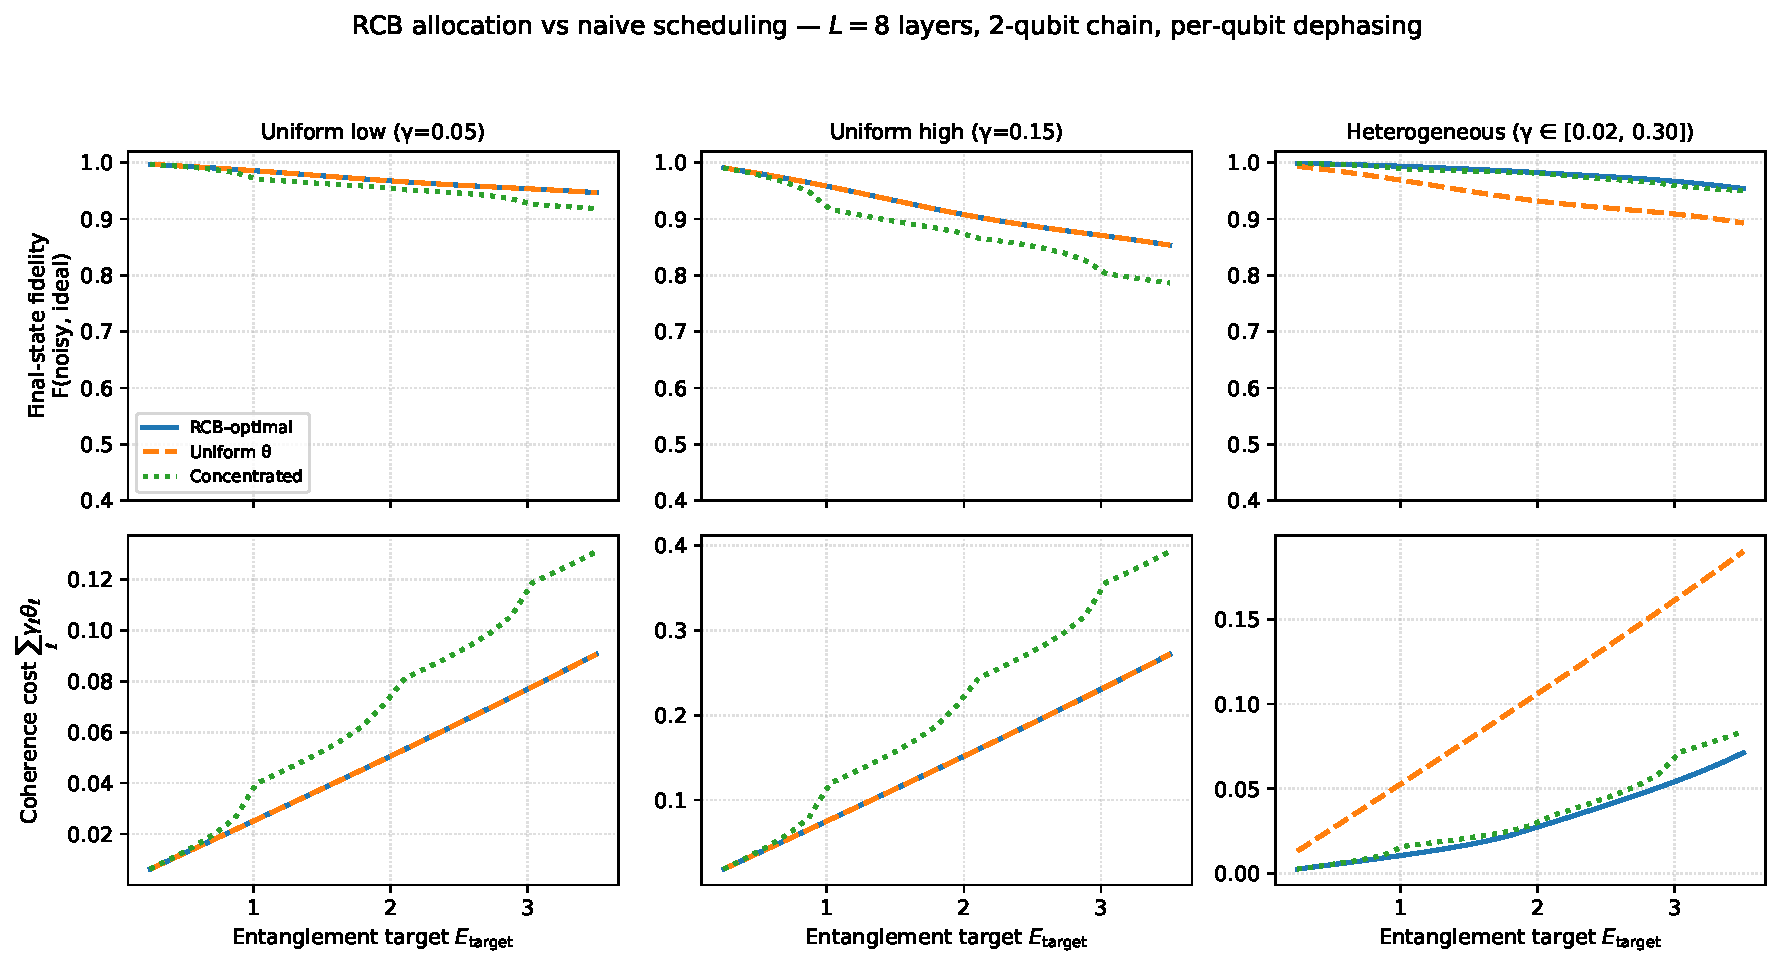
\includegraphics[width=0.9\textwidth]{fig3_rcb_sweep}
\caption{
  Coherence-Budget Allocation benchmark on an $L\!=\!8$ layer
  two-qubit circuit with per-layer independent pointer-basis dephasing.
  \textbf{Top row:} final-state fidelity vs noiseless target, as
  a function of entanglement target $E_{\rm target}$, for the RCB-optimal
  schedule (Eq.~\eqref{eq:alloc-solution}, solid),
  uniform-$\theta$ baseline (dashed), and concentrated full-entangler
  baseline (dotted).
  \textbf{Bottom row:} coherence cost
  $\sum_\ell \tilde\gamma_\ell\,\theta_\ell$ for the same schedules.
  \textbf{Columns:} uniform low noise
  ($\gamma\!=\!0.05$), uniform high noise ($\gamma\!=\!0.15$), and
  heterogeneous noise ($\gamma \in [0.02, 0.30]$).
  The RCB-optimal schedule equals or exceeds both baselines in
  fidelity across all $E_{\rm target}$; the largest advantage appears
  in the high-$\gamma$ regime (Prediction~P1) and in the
  heterogeneous regime against uniform $\theta$ (Prediction~P2).
  Generated by \texttt{figures/\allowbreak benchmark\_\allowbreak sweep.py}.
}
\label{fig:rcb-sweep}
\end{figure*}

P1 is visible in the uniform-$\gamma$ columns: distribution always
beats concentration.
P2 is visible in the heterogeneous column: RCB-optimal beats
uniform-$\theta$ by routing entanglement onto the
$\gamma\!=\!0.02$ layers and zero onto the $\gamma\!=\!0.30$ layer
(P3 in action).
The benchmark validates Theorem~\ref{thm:alloc} as a per-circuit,
not merely per-gate, statement of the coherence-budget framing.

\subsection{Layer-Varying Affinity}
\label{subsec:alpha-varying}

The benchmark above runs every layer at the same pre-gate affinity, and
in that regime $\bar\alpha$ drops out of the optimum: a common factor in
the effective rates $\tilde\gamma_\ell =
\bar\alpha_\ell^{\rm pre}\gamma_\ell\kappa$ is absorbed by the shadow
price (Sec.~\ref{subsec:limitations}, fifth limitation).
The \RCF~cost and a cost built from the dephasing rates alone differ only
when $\bar\alpha_\ell^{\rm pre}$ varies across layers, and this
subsection tests that regime (Fig.~\ref{fig:alpha-varying},
\texttt{figures/\allowbreak benchmark\_\allowbreak alpha\_\allowbreak varying.py}).
The circuits are the two-qubit, $L = 8$ circuits of
Sec.~\ref{subsec:benchmark-alloc}, with two additions that make
$\bar\alpha_\ell^{\rm pre}$ differ between layers: fixed single-qubit
rotations before each exchange layer, and idle dephasing between
layers that is common to every schedule.
The \RCF\ schedule takes $\bar\alpha_\ell^{\rm pre}$ from the noisy
trajectory of the rate-only schedule and then applies
Theorem~\ref{thm:alloc} once.
A self-consistent version, in which the profile is recomputed from the
schedule it produces, does not converge: the linear program moves all
of the entangling weight onto the lowest-affinity layers, which changes
the profile, and the iteration oscillates.
As a reference I maximize the simulated fidelity numerically under the
same constraint $\sum_\ell \sin 2\theta_\ell = E_{\rm target}$.

The results are mixed: when coherence decays steadily with depth, the \RCF\ schedule moves
the entangling angle onto the last layers and gains
$\Delta F = +0.022$ ($E_{\rm target} = 1$) and $+0.038$
($E_{\rm target} = 2$) over the rate-only schedule, most of what the
numerical optimum gains.
When the rotations make the affinity jump from layer to layer, the
schedule puts $\theta \approx 0.6$ on the single lowest-affinity
layer, well outside the small-angle regime in which
Eq.~\eqref{eq:linear-cost} holds, and loses $\Delta F = -0.035$.
Over 300 random circuits
($\gamma_\ell \in [0.02, 0.30]$, random rotations and idle
dephasing), the \RCF\ schedule beats the rate-only schedule on average
by $\Delta F = +0.003$ to $+0.005$ for
$E_{\rm target} \in \{0.5, 1, 2\}$ (standard errors 0.0005--0.0014),
but it is worse on 13--41\% of circuits and recovers only 10--25\% of
the gap to the numerical optimum, which is itself
$0.010$ to $0.052$.
Weighting each layer instead by the first-order infidelity
$\sum_{i\neq j} h_{ij}\,\lvert\rho_{ij}\rvert^2$ of the state exposed
to the gate noise, where $h_{ij}$ is the Hamming distance between
pointer states $i$ and $j$, recovers 23--38\%, although it fails in
the same way when the affinity jumps between layers.
That weight scales as $\bar\alpha^2$ rather than $\bar\alpha$, because
dephasing costs fidelity in proportion to the squared off-diagonal
elements.
The affinity is therefore operationally relevant, and the direction in
which it moves the schedule is right, but the linear-in-$\bar\alpha$
cost of Eq.~\eqref{eq:layer-cost} is not the best way to use it.

I tried the obvious repair: weight each layer by
$(\bar\alpha_\ell^{\rm pre})^2$ instead of $\bar\alpha_\ell^{\rm pre}$,
and add the bound $\theta_\ell \le \theta_{\max}$ to
Eq.~\eqref{eq:alloc-problem}.
The bound leaves Theorem~\ref{thm:alloc} intact; the optimal angle is
simply Eq.~\eqref{eq:alloc-solution} clipped at $\theta_{\max}$.
I chose $\theta_{\max} = \pi/12$ on a separate calibration set of 150
random circuits and then fixed it for the 300 reported above.
Of the two changes, the bound does most of the work.
In the case where the affinity jumps between layers, the capped
quadratic schedule gains $\Delta F = +0.019$ ($E_{\rm target} = 1$)
and $+0.027$ ($E_{\rm target} = 2$) where the linear schedule lost
$0.035$ and $0.039$; with steady decay it gives up a little
($+0.020$ and $+0.026$ instead of $+0.022$ and $+0.038$); and with
heterogeneous rates it gains $+0.011$ and $+0.012$.
Over the random circuits at $E_{\rm target} = 1$ it gains
$\Delta F = +0.013 \pm 0.002$, three times the linear schedule, recovers
43\% of the gap to the optimum instead of 14\%, and its worst single
loss falls from $0.11$ to $0.06$.
At $E_{\rm target} = 0.5$ the bound never binds and squaring the
weight adds little ($+0.003$).
At $E_{\rm target} = 2$ a fixed $\theta_{\max} = \pi/12$ is too
tight: meeting the target then forces angle onto at least four layers,
including noisy ones, and the gain falls to $+0.006$.
Squaring the weight without the bound barely changes the average and
makes the worst cases worse.
The lesson is that the coherence cost needs to stay inside the regime
in which it was derived, and that the bound should scale with
$E_{\rm target}/L$ rather than be fixed.
Even the best of these schedules recovers well under half of what
direct numerical optimization achieves, so a per-layer linear cost of
this kind, however it is weighted, remains an approximation.

\begin{figure*}[htbp]
\centering
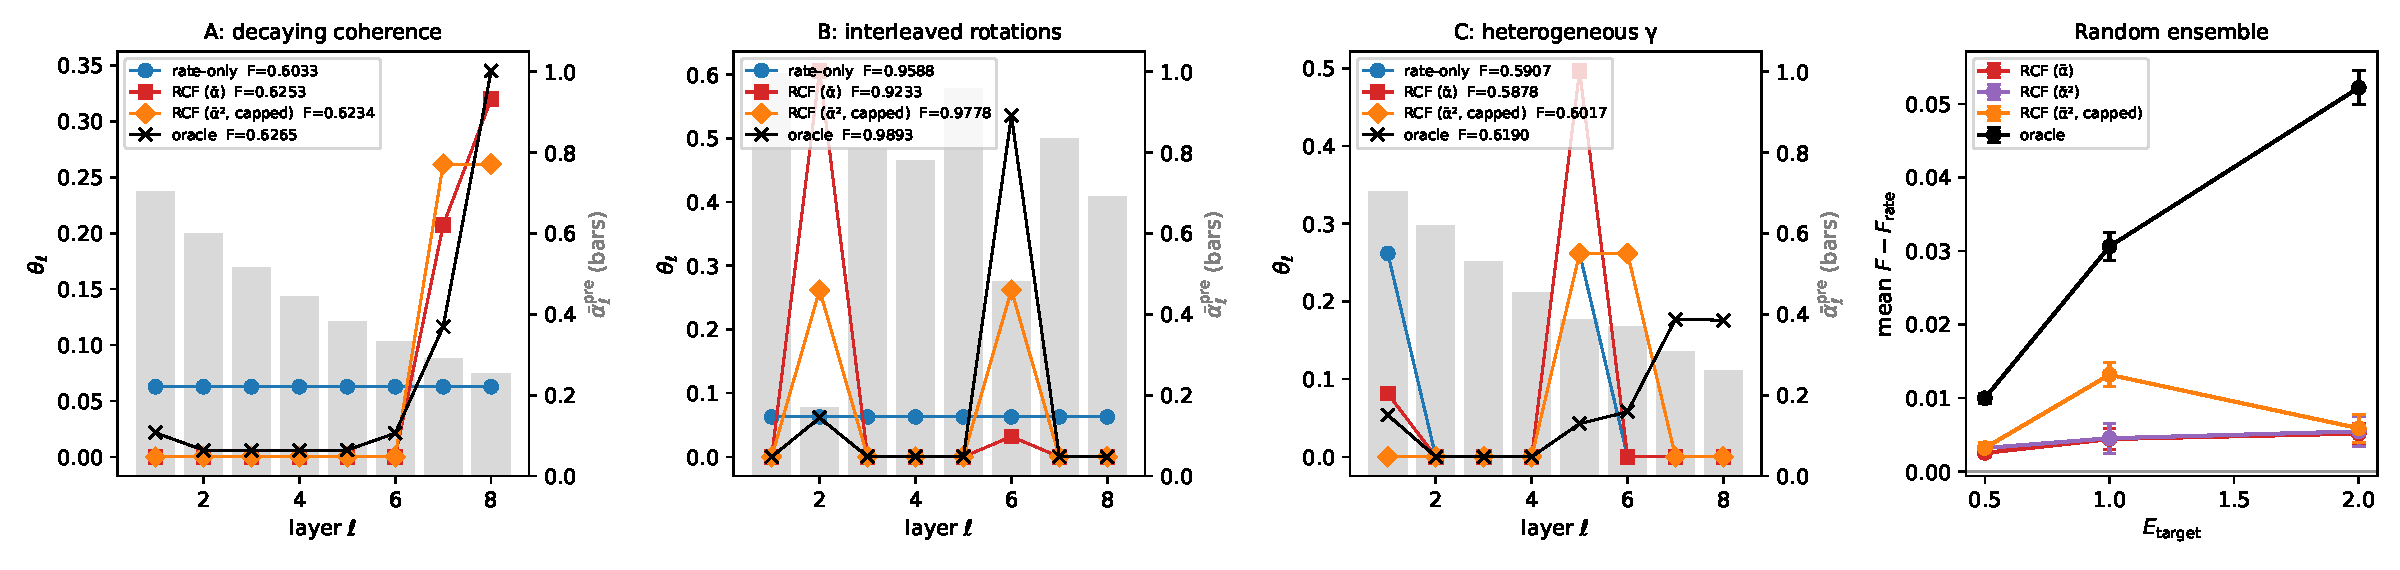
\includegraphics[width=\textwidth]{fig4_alpha_varying}
\caption{
  Allocation with layer-varying pre-gate affinity ($L = 8$,
  $E_{\rm target} = 1$ in the first three panels).
  Gray bars: $\bar\alpha_\ell^{\rm pre}$ along the rate-only schedule.
  Lines: exchange angles $\theta_\ell$ for the rate-only schedule,
  the \RCF\ schedule ($\tilde\gamma_\ell \propto
  \bar\alpha_\ell^{\rm pre}\gamma_\ell$), the capped quadratic
  schedule ($\tilde\gamma_\ell \propto
  (\bar\alpha_\ell^{\rm pre})^2\gamma_\ell$,
  $\theta_\ell \le \pi/12$), and the numerical optimum, with final-state fidelities
  in the legends.
  \textbf{A:} uniform $\gamma = 0.15$, coherence decaying through idle
  dephasing.
  \textbf{B:} uniform $\gamma = 0.15$, interleaved single-qubit
  rotations.
  \textbf{C:} the heterogeneous rates of Fig.~\ref{fig:rcb-sweep}
  with idle dephasing.
  \textbf{Right:} mean fidelity gain over the rate-only schedule
  across 300 random circuits (error bars: standard error).
  Generated by \texttt{figures/\allowbreak benchmark\_\allowbreak alpha\_\allowbreak varying.py}.
}
\label{fig:alpha-varying}
\end{figure*}

\subsection{Scope of Theorem~\ref{thm:alloc}}
\label{subsec:alloc-scope}

The allocation theorem holds under the assumptions made explicit in
Sec.~\ref{sec:sim}: (i)~Markovian pure-dephasing dynamics in the
einselected pointer basis, with rates that are constant within each
gate window;
(ii)~gate-time-proportional coherence-limited error (small-$p$
leading-order linearization of Eq.~\eqref{eq:peff});
(iii)~direct exchange calibration so that $\URA(\theta)$ is realized
as a single tunable pulse rather than decomposed into fixed native
gates.
Where (iii) fails, the constant $\kappa$ relating $\theta$ to
duration in Eq.~\eqref{eq:layer-cost} is replaced by a
decomposition-depth--dependent factor; the optimization problem and
its solution form are unchanged but the numerical advantage shrinks
as in Sec.~\ref{sec:disc}.
Coherent calibration errors, leakage to non-computational levels, and
crosstalk are not modelled by Eq.~\eqref{eq:peff} and can shift the
optimum; their incorporation as additional per-layer cost terms is
straightforward and preserves the convex-program structure.

% ── SECTION 6: DISCUSSION (~1,200 words) ─────────────────────────────────────

\section{Discussion}
\label{sec:disc}

\subsection{The Affinity Operator and Existing Coherence Measures}

The scalar affinity $\bar\alpha(S,E)$ is a measure of \emph{local}
quantum coherence~---~the off-diagonal magnitude of the reduced state
$\rho_S$ in the einselected pointer basis~---~and it is therefore a
distinct object from standard bipartite entanglement measures.
Concurrence~\cite{Wootters1998} and von Neumann
entropy~\cite{vonNeumann1932} quantify the entanglement of the joint
state $\rho_{SE}$; $\bar\alpha$ quantifies the residual pointer-basis
superposition that environmental monitoring has not yet resolved into a
definite outcome (Proposition~\ref{prop:indefiniteness}).
The two are not equal even on two-qubit pure states: a Bell state
$\ket{\Phi^+}$ has reduced state $\rho_S = \mathbf{I}/2$, hence
$\bar\alpha = 0$ and concurrence $\mathcal{C} = 1$, while a product
superposition $\ket{+}_S\otimes\ket{0}_E$ has $\bar\alpha = 1$ and
$\mathcal{C} = 0$ (cf.\ the Affinity-vs.-Entanglement remark in
Sec.~\ref{sec:prop3} and the explicit computation in
App.~\ref{app:rct-proof}).

Along the dephasing trajectory of Proposition~\ref{prop:determination}
the two measures are inversely related: as the conditional environmental
branches in Eq.~\eqref{eq:coherence-transfer} become orthogonal,
$\bar\alpha(t) \to 0$ while the $S$-$E$ entanglement entropy $S(\rho_S)$
saturates at the Shannon entropy of the pointer-basis populations
$\{\lvert c_k\rvert^2\}$,
$-\sum_k \lvert c_k\rvert^2 \log \lvert c_k\rvert^2$, which equals
$\log d$ only for the equal-weight initial state $\bar\alpha(0) = 1$
(Proposition~\ref{prop:conservation}, parts~(ii) and~(iii)).
This complementary relationship is what makes $\bar\alpha$ useful as a
dynamical figure of merit.
Concurrence and entropy report on a static joint state at one moment;
$\bar\alpha(t)$ reports on the time-evolving local coherence budget that
remains available to a unitary acting on $S$ alone.
For circuit-level coherence accounting~---~quantifying how much
pointer-basis coherence a gate consumes, layer by layer, before the
bath records it~---~the appropriate observable is $\bar\alpha$, not
concurrence.

\subsection{Relation to the Resource Theory of Coherence}
\label{subsec:rtoc}

The scalar affinity sits naturally alongside the basis-dependent
quantifiers of the resource theory of coherence developed by
Baumgratz, Cramer, and Plenio~\cite{Baumgratz2014} and surveyed in
\cite{Streltsov2017Review}.
That framework fixes a reference basis $\{\vert i\rangle\}$, designates
the basis-diagonal states as incoherent, and characterizes coherence
through monotones such as the
$\ell_1$-norm of coherence
$C_{\ell_1}(\rho) = \sum_{i\neq j}\lvert\rho_{ij}\rvert$ and the
relative entropy of coherence
$C_{\rm re}(\rho) = S(\rho_{\rm diag}) - S(\rho)$.
The scalar affinity is the normalized Hilbert--Schmidt quantifier in the
same family,
$\bar\alpha^2(\rho_S) = (d/(d-1))\sum_{i\neq j}\lvert\rho_{ij}\rvert^2$,
and it shares the structural features that define the family: it
vanishes precisely on the incoherent (basis-diagonal) states
[Prop.~\ref{prop:correspondence}(i)] and attains its maximum on the
equal-weight basis superposition [Prop.~\ref{prop:correspondence}(ii)],
the same extremes as $C_{\ell_1}$ and $C_{\rm re}$.
I do not claim $\bar\alpha$ is a coherence monotone in the strict
sense of~\cite{Baumgratz2014}; the Hilbert--Schmidt quantifier is not
in general monotone under arbitrary incoherent CPTP maps, and the
use of $\bar\alpha$ here is as a circuit-level figure of merit
under physical (Markovian dephasing, gate-time-proportional)
noise channels, where its monotonic decay
[Prop.~\ref{prop:determination}] is exact.

What the \RCF~adds that the resource-theory framework does not supply
on its own is twofold.
First, the reference basis is not stipulated~---~it is fixed by
physics: einselection (Sec.~\ref{sec:decoherence}) singles out the
pointer basis from the $S$-$E$ Hamiltonian, so the basis-dependence of
$\bar\alpha$ is grounded in the dynamics rather than chosen by
convention.
Second, $\bar\alpha$ acquires a conservation-law interpretation under
unitary $S{+}E$ evolution [Prop.~\ref{prop:conservation}]: the local
coherence depleted from $\rho_S$ is redistributed into $S$-$E$
correlations rather than annihilated.
The resource-theory monotones quantify static coherence relative to a
chosen basis; $\bar\alpha$ is a kindred quantifier placed in a
dynamical, conservation-aware, einselection-grounded setting.

This redistribution-rather-than-annihilation reading has recently
acquired a vivid physical illustration outside the circuit setting.
Yuksel et al.~\cite{Yuksel2026PhononicDressed} tune a nanomechanical
resonator into resonance with a single intrinsic two-level
defect~---~ordinarily regarded as a decoherence channel~---~and recover
the would-be-lost coherence as a hybridized phononic ``dressed state,''
so that a single defect that one system--environment partition registers
as irreversible decoherence another addresses as a coherent relational
partner.
I record this as illustration, not evidence: it occupies the
strong-coupling, non-Markovian regime outside the Markovian,
einselection-grounded scope in which $\bar\alpha$ is defined here
(cf.\ the Markovian-dephasing premise of Prop.~\ref{prop:determination}
and the einselection idealization of Def.~\ref{def:alpha-tensor}), and
the quantitative claims of the \RCF~are neither confirmed nor
presupposed by it.

\subsection{Relation to Noise-Aware Compilation for Continuously Parameterized Gates}
\label{subsec:prior-compilation}

Recent noise-aware compilation work for continuously parameterized two-qubit gates
has demonstrated hardware-level results qualitatively consistent with the predictions
of Theorem~\ref{thm:alloc}.
Yale et al.~\cite{Yale2025NoiseAware} implement noise-aware compilations on a
trapped-ion QSCOUT processor using continuously parameterized $\mathcal{ZZ}$ gates
(M\o{}lmer--S\o{}rensen interaction) through the Superstaq compiler platform,
and show that compiler optimizations can reduce total entangling angle, assign
heavier $\mathcal{ZZ}$-angle participation to better-performing qubit pairs, and
remove the least impactful $\mathcal{ZZ}$ operations to improve circuit fidelity.
These empirical observations correspond qualitatively to Predictions~P2 and~P3
of Theorem~\ref{thm:alloc}: heavier entangling weight is routed toward quieter
gate pairs~(P2), and gates whose marginal fidelity contribution is below threshold
are zeroed out~(P3).

The present work is complementary in both derivation and scope.
Yale et al.\ begin from calibrated hardware performance data and apply
compiler heuristics optimized for the trapped-ion $\mathcal{ZZ}$ (Mølmer--Sørensen)
gateset on QSCOUT; their central result is empirical validation that such
optimizations improve quantum volume on real hardware.
The \RCF~begins instead from a pointer-basis coherence-cost functional
$\mathcal{C}_{\RCF}(\mathcal{U})$ (Eq.~\eqref{eq:circuit-cost}), derived from
the einselection-grounded scalar affinity $\bar\alpha$ via
Proposition~\ref{prop:determination}, and derives a \emph{closed-form}
exchange-angle allocation rule (Eq.~\eqref{eq:alloc-solution}) from
KKT optimality conditions on that functional.
To my knowledge, prior noise-aware compilation work for continuously
parameterized two-qubit gates has arrived at qualitatively similar routing
and skipping behaviours through compiler search over calibrated hardware metrics.
The contribution claimed here is not the use of continuous gates, noise-aware
angle routing, or the omission of low-impact operations~---~all demonstrated
in~\cite{Yale2025NoiseAware}~---~but the derivation of those behaviours as the
unique analytic solution to a convex coherence-budget program grounded in
einselection.

\subsection{The Gate-Time Advantage and its Interpretation}

The simulation results of Sec.~\ref{sec:sim} are an
$\bar\alpha$-language expression of a now-established hardware
observation: on platforms where the two-qubit-gate pulse duration is
set by the Heisenberg exchange coupling, partial-exchange gates
accumulate less coherence-limited error than fixed maximally-entangling
gates, with the fidelity savings demonstrated experimentally for the
continuous fSim and parametric-exchange families by Foxen,
Abrams, Lacroix, and others~\cite{Foxen2020,Abrams2020,Lacroix2020,Caldwell2018}.
My independent simulations recover this in
$\bar\alpha$-language: at $\theta < \pi/4$, $\URA(\theta)$ accumulates
a smaller fraction of the per-gate decoherence budget than a fixed
maximally-entangling primitive [Eq.~\eqref{eq:peff}], equivalently
redistributing a smaller fraction of the local pointer-basis coherence
$\bar\alpha$ into $S$--bath correlations.
The fidelity advantage~---~$\Delta F \in [+0.038,+0.039]$ at
$p_{\rm base} = 0.10$ across depolarizing, dephasing, and amplitude
damping noise, growing from $\Delta F \in [+0.019,+0.020]$ at
$p_{\rm base} = 0.05$ (Table~\ref{tab:fidelity-all})~---~is the
cumulative result of this per-gate saving over a circuit.

I stress what this result is and is not.
It is \emph{not} a quantitative identity between $\theta$ and
$\bar\alpha$; the exchange angle and the scalar affinity have different
domains and inverse responses, as discussed in Sec.~\ref{sec:gate}.
What the \RCF~contributes is the coherence-budget framing for the
parameter selection: the redistribution structure of
Proposition~\ref{prop:conservation} renders the per-gate cost of
partial entanglement explicit as a fraction of $\bar\alpha$ exported into
$S$--$E$ correlations, and the gate-time-proportional noise model of
Eq.~\eqref{eq:peff} combined with the continuous Weyl-chamber
trajectory $(c_1,c_2,c_3)=(\theta,\theta,\theta)$
(Sec.~\ref{subsec:weyl}) then yields the corresponding average-gate
fidelity advantage.
I claim independent simulation consistency with the experimental
continuous-fSim advantage, not novelty for the underlying hardware
observation.

\paragraph{Practical shot-count implication.}
The per-gate fidelity advantage $\Delta F = (3/8)\,p_{\rm base}$
(Table~\ref{tab:fidelity-all}) compounds across circuit depth.
For a circuit of $n$ coherently applied exchange layers, the
final-state success probability scales as $p_s \approx F^n$, and the
number of measurement shots required to collect $k$ successful
outcomes is $N_{\rm shots} = k/p_s$.
The ratio of shots required under the fixed-gate versus RCB-optimal
schedule is therefore
%
\begin{equation}
\label{eq:shot-ratio}
\frac{N_{\rm shots}^{\rm fixed}}{N_{\rm shots}^{\rm RCB}}
  \;=\; \left(\frac{F_{\rm RCB}}{F_{\rm fixed}}\right)^{\!n}.
\end{equation}
%
At $p_{\rm base} = 0.10$ and $n = 8$ layers,
$F_{\rm RCB} = 0.9625$ and $F_{\rm fixed} = 0.9250$ per gate
(Table~\ref{tab:fidelity}), giving $F_{\rm RCB}^8 / F_{\rm fixed}^8
\approx 0.736 / 0.536 \approx 1.37$: the fixed-gate circuit requires
roughly $37\%$ more measurement shots to achieve the same sampling
statistics.
At $p_{\rm base} = 0.05$ the ratio falls to approximately $1.16$.
These estimates assume multiplicative, gate-time-proportional error
accumulation (the regime of Eq.~\eqref{eq:peff}) and do not model
readout error or inter-layer correlations; they restate the fidelity
advantage of Theorem~\ref{thm:alloc} in resource-accounting terms
directly relevant to algorithm-level cost benchmarks.

\subsection{Scope and Limitations}

The \RCF~formalizes the relational structure of quantum mechanics
established by Bell's theorem~\cite{Bell1964} and relational quantum
mechanics~\cite{Rovelli1996,Rovelli2021}; it does not resolve the
quantum measurement problem.
It provides a precise formal vocabulary within which a definite outcome
is described as the establishment of a relational fact under
einselection (Proposition~\ref{prop:determination}, operational
corollary in App.~\ref{app:rct-proof}), but the question of
\emph{which} outcome is selected in a given experimental run remains
outside the framework's scope, as it does for all no-collapse
interpretations.

Five further limitations bound the simulation claims.
First, the gate-time-proportional noise model (Eq.~\eqref{eq:peff})
captures only the coherence-limited contribution to gate error and is
appropriate for Heisenberg exchange directly calibrated on suitable
hardware~\cite{LossDiVincenzo1998,Krantz2019,Caldwell2018,Foxen2020,Abrams2020};
coherent calibration error, leakage to non-computational levels, and
spectator-qubit crosstalk can scale differently with $\theta$ and may
attenuate the advantage at small $\theta$.
On platforms where $\URA(\theta)$ must be decomposed into fixed native
gates~\cite{VatanWilliams2004}, the fidelity advantage depends on the
decomposition depth and may shrink or vanish.
Second, the calibration overhead of providing $\URA(\theta)$ at
arbitrary $\theta$~---~either as continuous in-situ tuning or as a
pre-calibrated lookup~---~is not modelled here and constitutes an
additional engineering cost that may offset per-gate savings in
algorithm-level benchmarks~\cite{Foxen2020,Lacroix2020}.
Third, the decoherence treatment of Proposition~\ref{prop:determination}
adopts the Markovian approximation; non-Markovian environments introduce
memory kernels that modify the $e^{-\gamma t}$ decay law without
qualitatively altering the redistribution result of
Proposition~\ref{prop:conservation}, but a quantitative extension is
deferred to future work.
Fourth, the einselection idealization assumed in
Definition~\ref{def:alpha-tensor} is sharp only in the limit in which
the pointer basis has converged; for finite baths and finite times the
pointer basis is approximate, time-dependent, and partially defined,
and the basis-dependence of $\bar\alpha$ inherits this
approximation~\cite{Schlosshauer2005}.
The relational network $\Gamma_S$ is also treated here as a collection
of interaction events rather than a weighted graph; coupling-strength
and event-ordering effects on the multi-environment generalization are
left to subsequent development (cf.\ Sec.~\ref{sec:rqm}).
Fifth, the scalar affinity enters the allocation program of
Theorem~\ref{thm:alloc} only through the effective rates
$\tilde\gamma_\ell = \bar\alpha_\ell^{\rm pre}\gamma_\ell\kappa$
(Eq.~\eqref{eq:linear-cost}), and the optimal schedule
Eq.~\eqref{eq:alloc-solution} is invariant under a common rescaling
$\tilde\gamma_\ell \to c\,\tilde\gamma_\ell$ ($c>0$), which is absorbed
exactly by the shadow price $\lambda^{\!*} \to c\,\lambda^{\!*}$.
Consequently, when the pre-gate affinity is the same on every layer,
$\bar\alpha$ drops out of the argmin and the schedule depends only on
the dephasing rates $\gamma_\ell$ and on $E_{\rm target}$.
The benchmarks of Sec.~\ref{subsec:benchmark-alloc} are run in this
regime (the reference scheduler takes the rates $\gamma_\ell$ directly),
so the present numerics do not discriminate between the \RCF~cost
functional and a cost built from the dephasing rates alone.
The two differ only when $\bar\alpha_\ell^{\rm pre}$ varies across
layers~---~for example, as residual coherence decays through a deep
circuit~---~in which case the \RCF~schedule shifts entangling weight
toward layers that retain more pointer-basis coherence.
Testing that layer-dependent regime, in which the einselection-derived
affinity is operationally load-bearing, is left to future work.

\subsection{Decomposition Break-Even for Fixed-Gate Platforms}
\label{subsec:decomp-breakeven}

On platforms where $\URA(\theta)$ is not directly calibrated but must
instead be synthesized from a fixed native gateset, the gate-time
proportionality of Eq.~\eqref{eq:peff} is replaced by a
decomposition-depth cost.
$\URA(\theta)$ (Eq.~\eqref{eq:URA-matrix}) is \emph{not} a purely real
(SO(4)-equivalent) unitary for any $\theta \in (0,\pi/4]$: its triplet
block carries the overall phase $e^{-i\theta/2}$ while its
$\{\ket{01},\ket{10}\}$ block carries $e^{i\theta/2}$, and no single
global phase can render both real simultaneously except at $\theta = 0$.
Consequently the $N_{\rm CNOT} = 2$ special case of the KAK
decomposition~\cite{VatanWilliams2004} --- which applies only to gates
locally equivalent to a real (SO(4)) unitary --- does not apply here;
the relevant bound is instead the generic
$N_{\rm CNOT} = 3$ result, shown to be necessary and
sufficient for a generic $\mathrm{SU}(4)$ gate by
Vidal and Dawson~\cite{VidalDawson2004}.
We confirmed numerically, via exact synthesis
(\texttt{TwoQubitBasisDecomposer} in Qiskit and an independent
Makhlin-invariant calculation~\cite{Makhlin2002}), that $\URA(\theta)$
requires exactly 3 CNOT gates for every $\theta \in (0,\pi/4]$ tested,
including the boundary and near-zero limits; no compilation route
reduces this to 2 for a generic angle in this family.
Each CNOT contributes error $p_{\rm CNOT}$ independently of $\theta$,
so the effective fidelity of the decomposed gate is
%
\begin{equation}
\label{eq:fidelity-decomp}
F_{\rm decomp}
  \;\approx\; (1 - p_{\rm CNOT})^3
  \;\approx\; 1 - 3\,p_{\rm CNOT},
\end{equation}
%
while the directly calibrated $\URA(\theta)$ achieves
$F_{\rm direct}(\theta) = 1 - \tfrac{3}{4}\,p_{\rm base}\cdot\theta/(\pi/4)$
(Table~\ref{tab:fidelity}, depolarizing column).
Setting $F_{\rm direct}(\theta) \geq F_{\rm decomp}$ yields the
\emph{decomposition break-even condition}: direct calibration retains
its fidelity advantage over the decomposed implementation if and only if
%
\begin{equation}
\label{eq:breakeven}
p_{\rm CNOT}
  \;<\; \frac{1}{4}\cdot\frac{\theta}{\pi/4}\cdot p_{\rm base}.
\end{equation}
%
At the half-entangling point $\theta = \pi/8$ and
$p_{\rm base} = 0.10$, the threshold is
$p_{\rm CNOT}^{\rm BE} = (1/8)\times 0.10 = 0.0125$.
Current best-reported two-qubit gate error rates on superconducting
and trapped-ion hardware range from $p_{\rm CNOT} \approx 0.003$
to $0.015$~\cite{Krantz2019}, which now straddles this threshold rather
than sitting uniformly below it: only the lower half of this range
($p_{\rm CNOT} \lesssim 0.0125$) retains the direct-calibration
advantage at $\theta=\pi/8$, and the break-even threshold scales
linearly with $\theta$, so smaller exchange angles shrink the safe
range further (e.g.\ at $\theta = \pi/16$, the threshold falls to
$0.00625$, already below most reported hardware error rates).
On platforms or operating points where $p_{\rm CNOT} > p_{\rm
CNOT}^{\rm BE}(\theta)$~---~which now includes a meaningful fraction of
present-day devices at partial-exchange operating points, not only
older or crosstalk-limited hardware~---~the decomposition overhead
erases the gate-time saving and the fixed-gate baseline should be
preferred.
Equation~\eqref{eq:breakeven} thus converts the qualitative limitation
noted above into a testable, hardware- and angle-specific criterion,
one that is markedly less permissive than a naive $N_{\rm CNOT}=2$
assumption would suggest.

\subsection{Future Directions}

Three extensions are immediate.
First, experimental implementation of $\URA(\theta)$ on superconducting
qubit platforms~\cite{Krantz2019} via direct calibration of the
Heisenberg exchange coupling, bypassing gate-decomposition overhead.
Second, extension to multi-qubit relational networks: generalizing the
Affinity Operator to $n$-qubit systems $\alpha(S,\{E_i\})$ and deriving
the corresponding $n$-qubit Relational Affinity unitaries parameterized
by the full tensor, with attention to the weighted-graph $\Gamma_S$
deferred above.
Third, investigation of $\bar\alpha$-aware quantum error correction:
the local pointer-basis coherence budget may provide a natural
diagnostic for surface-code threshold behaviour distinct from the usual
logical-error rate.
The philosophical implications of the \RCF~---~including the argument
that process ontology is formally required (not merely permitted) by
quantum mechanics~---~are developed in the companion
paper~\cite{Adams2026Philosophy}.

% ── SECTION 7: CONCLUSION (~500 words) ───────────────────────────────────────

\section{Conclusion}
\label{sec:conc}

I have introduced the Relational Coherence framework (\RCF), a
formal packaging of the relational reading of quantum
mechanics~\cite{Bell1964,Rovelli1996,Rovelli2021} into a single
computable scalar quantity~---~the scalar affinity
$\bar\alpha(S,E)$, the normalized Hilbert--Schmidt coherence of
$\rho_S$ in the einselected pointer
basis~\cite{Zurek2003,Baumgratz2014,Streltsov2017Review}.
The \RCF~comprises four propositions~---~property indefiniteness,
relational determination, coherence--affinity correspondence, and
coherence redistribution under unitary $S$--$E$ evolution~---~each of
which rests on standard quantum-mechanical machinery (Cauchy--Schwarz
bounds, Lindblad calculation, Schmidt decomposition, Joos--Zeh / Zurek
branching) packaged in $\bar\alpha$-language; the framework's
contribution lies in this packaging, not in the underlying identities.

The Affinity Operator~$\alpha(S,E)$ provides an operationalized, computable
measure of relational coherence: it is built from the off-diagonal
entries of the reduced state $\rho_S$ in the einselected pointer basis,
and so quantifies \emph{local} pointer-basis coherence rather than $S$-$E$
entanglement (Proposition~\ref{prop:correspondence} and the remark on
affinity vs.\ entanglement in Sec.~\ref{sec:prop3}).
Under environmental noise, $\bar\alpha(t)$ tracks the quantum-to-classical
transition as a single scalar trajectory, decaying from maximal local
coherence ($\bar\alpha = 1$, an equal-weight pointer-basis superposition)
to a pointer-basis-diagonal classical mixture ($\bar\alpha = 0$) while
total purity is conserved in the joint $S{+}E$ system
(Proposition~\ref{prop:conservation}).

The gate~$\URA(\theta)$ examined in this work is the well-known
isotropic Heisenberg-exchange family, characterized by Weyl-chamber
coordinates $(c_1, c_2, c_3) = (\theta, \theta, \theta)$, examined here
in the coherence-budget framing supplied by the
\RCF~\cite{LossDiVincenzo1998,Zhang2003WeylChamber,Foxen2020,Abrams2020,Lacroix2020,Caldwell2018}.
The exchange angle $\theta$ is a Hamiltonian evolution parameter, not a
direct identification with $\bar\alpha$; what the \RCF~contributes is
the per-layer coherence-budget reading of the parameter selection, with
Proposition~\ref{prop:conservation} rendering the per-gate cost of
partial entanglement explicit as a fraction of $\bar\alpha$ exported
into $S$--$E$ correlations.
Numerical simulation under gate-time-proportional depolarizing,
dephasing, and amplitude damping noise yields, for $\URA(\pi/8)$
operating at half the duration of a full \textsc{iswap} or \textsc{cnot},
fidelity advantages of $\Delta F \in [+0.038, +0.039]$ over fixed gates
at $p_{\rm base} = 0.10$ (and $\Delta F \in [+0.019, +0.020]$ at
$p_{\rm base} = 0.05$), consistent with and quantitatively similar to
the experimental continuous-fSim advantage reported on
Sycamore-class hardware by Foxen~\textit{et~al.}~\cite{Foxen2020}.

These results illustrate the \RCF~as a formal packaging: the Affinity
Tensor is computable from the reduced state in the einselected pointer
basis, the gate is implementable on platforms with directly
calibratable exchange coupling, and the simulated fidelity advantage
under gate-time-proportional decoherence is the analytical consequence
of the gate-time scaling combined with the continuous Weyl-chamber
trajectory.

The principal technical contribution of this paper is the
\emph{Coherence-Budget Allocation Theorem} (Sec.~\ref{sec:alloc}), which
turns the per-gate coherence-budget framing into a layerwise scheduling
rule with a unique closed-form solution
$\theta_\ell^\ast = \tfrac{1}{2}\arccos\bigl(\min(1,\tilde\gamma_\ell/(2\lambda^\ast))\bigr)$.
The theorem yields three falsifiable predictions~---~distribute
entanglement rather than concentrate it, route entanglement onto
quieter layers, and skip layers whose effective dephasing rate
exceeds the global shadow price~---~which a reference scheduler
(\texttt{figures/rcb\_optimizer.py}) verifies on a multi-layer 2-qubit
benchmark.
Against a concentrated full-entangler baseline the optimal schedule
yields a final-state fidelity advantage of up to $\Delta F = +0.040$ at
$\gamma = 0.15$, $E_{\rm target}\!=\!1$, $L\!=\!8$; against
uniform-$\theta$ on heterogeneous noise it yields $\Delta F = +0.025$
at the same target.

I make no novelty claim for the gate itself, nor for the underlying
identities of the four propositions; the framework's utility is the
$\bar\alpha$-language diagnostic and the allocation theorem it
supports as a circuit-level scheduling rule.

Philosophical implications of the relational reading are deferred to
the companion paper~\cite{Adams2026Philosophy}.

\section*{Code and Data Availability}

All simulation scripts and figure-generation code used in this work are
publicly available at
\url{https://github.com/dradams-lab/pub1-physics-rct} and archived
at Zenodo, concept DOI~\texttt{10.5281/\allowbreak zenodo.20130304} (evergreen).
The repository includes:
\texttt{figures/\allowbreak generate\_\allowbreak fig1.py} (single-qubit affinity decay,
Fig.~\ref{fig:affinity-decay});
\texttt{figures/\allowbreak generate\_\allowbreak fig2.py} (two-qubit independent-dephasing
dynamics, Fig.~\ref{fig:alpha-dynamics});
\texttt{figures/\allowbreak generate\_\allowbreak tables.py} (closed-form analytical
reproduction of Tables~\ref{tab:fidelity}--\ref{tab:fidelity-all});
and the density-matrix simulator scripts
\texttt{figures/\allowbreak simulate\_\allowbreak table2\_\allowbreak qiskit.py} and
\texttt{figures/\allowbreak simulate\_\allowbreak table2\_\allowbreak cirq.py}, which reproduce the
dephasing and amplitude-damping rows of
Table~\ref{tab:fidelity-all} via independent full-channel simulation
in Qiskit-Aer and Cirq and agree with the analytical values to
numerical precision.


% ── Appendix ──────────────────────────────────────────────
\appendix
% ── APPENDIX A: FULL RCF PROOFS ──────────────────────────────────────────────

\section{Full Proofs for the Relational Coherence Framework}
\label{app:rct-proof}

\subsection{Mathematical Preliminaries}

Let $\mathcal{H}_S$ and $\mathcal{H}_E$ be finite-dimensional Hilbert spaces
with $\dim\mathcal{H}_S = d_S \geq 2$ and $\dim\mathcal{H}_E = d_E \geq d_S$.
The composite system occupies $\mathcal{H} = \mathcal{H}_S \otimes \mathcal{H}_E$.
Observables are self-adjoint elements of the C*-algebra
$\mathcal{B}(\mathcal{H})$ of bounded linear operators on $\mathcal{H}$.
States are density operators: positive trace-class operators
$\rho \in \mathcal{B}(\mathcal{H})$ with $\mathrm{Tr}[\rho] = 1$.

Fix orthonormal bases $\{\ket{s_i}\}_{i=1}^{d_S}$ and
$\{\ket{e_k}\}_{k=1}^{d_E}$ for $\mathcal{H}_S$ and $\mathcal{H}_E$
respectively.
Any pure state of $SE$ admits the Schmidt decomposition
\begin{equation}
  \ket{\psi_{SE}} = \sum_{j=1}^{r} \sqrt{\lambda_j}\,\ket{u_j}\otimes\ket{v_j},
  \label{eq:schmidt}
\end{equation}
where $r \leq \min(d_S, d_E)$ is the Schmidt rank, $\lambda_j > 0$,
$\sum_j \lambda_j = 1$, and $\{\ket{u_j}\}$, $\{\ket{v_j}\}$ are
orthonormal sets in $\mathcal{H}_S$ and $\mathcal{H}_E$ respectively.
The state is a product state iff $r = 1$; it is maximally entangled iff
$r = \min(d_S, d_E)$ and all $\lambda_j = 1/r$.

\subsection{Proof of Proposition~\ref{prop:indefiniteness} (Property Indefiniteness)}

The proposition statement in Sec.~\ref{sec:prop1} is the
linear-algebraic fact that $\bar\alpha(S,E)>0$ implies a non-diagonal
$\rho_S$ in the pointer basis, and that proof appears in
Sec.~\ref{sec:prop1}.
The Bell / Kochen--Specker material below is the auxiliary
no-hidden-variables result that supplies the physical content of
property indefiniteness against \emph{local non-contextual} hidden
variables; it is not a proof of the proposition as stated, but the
foundational anchor that justifies reading a non-diagonal $\rho_S$ as
the absence of a definite outcome rather than as ignorance of one.

\textbf{Auxiliary claim (no local non-contextual hidden variables).}
There is no \emph{local, non-contextual} value assignment
$v: \mathcal{O}(\mathcal{H}_S) \to \mathbb{R}$
mapping each self-adjoint observable $\hat{A}$ on $\mathcal{H}_S$ to a
definite eigenvalue $v(\hat{A}) \in \mathrm{spec}(\hat{A})$
consistently with all quantum predictions.
(Nonlocal hidden-variable theories such as Bohmian
mechanics~\cite{Bohm1980} evade this conclusion by accepting explicit
nonlocality; the result below constrains only local non-contextual
assignments.)

\textbf{Proof.}
I treat the two cases $d_S = 2$ and $d_S \geq 3$ separately.

\textit{Case $d_S = 2$ (qubit).}
Suppose, for contradiction, that definite pre-existing values
$A, A', B, B' \in \{+1,-1\}$ exist for all qubit observables and
depend only on local measurement settings.
The algebraic identity $|AB - AB' + A'B + A'B'| \leq 2$ holds for any
four such values, and averaging over the hidden-variable distribution
preserves the bound: for any joint state of two qubits and measurement
directions $\mathbf{a}, \mathbf{a}', \mathbf{b}, \mathbf{b}'$, the
CHSH combination satisfies
\begin{equation}
  \bigl|\langle\hat{A}\hat{B}\rangle - \langle\hat{A}\hat{B}'\rangle
    + \langle\hat{A}'\hat{B}\rangle + \langle\hat{A}'\hat{B}'\rangle\bigr|
  \leq 2.
\end{equation}
For the maximally entangled state $\ket{\Phi^+}$ with directions chosen at
$45^\circ$ intervals, quantum mechanics predicts a violation up to the
Tsirelson bound $2\sqrt{2}$~\cite{Tsirelson1980}, confirmed
experimentally~\cite{Aspect1982,Zeilinger2022Nobel}.
This contradiction establishes that no pre-existing value assignment exists
for $d_S = 2$.

\textit{Case $d_S \geq 3$.}
The Kochen--Specker theorem~\cite{KochenSpecker1967} proves that for
$d_S \geq 3$, there is no non-contextual hidden variable assignment
consistent with the quantum predictions for all projection-valued
measures on $\mathcal{H}_S$.
(A non-contextual assignment would give the same value to a projector
$\hat{P}$ regardless of which complete set of commuting observables it
is measured alongside~--- precisely the assignment required by any
hidden variable theory seeking to recover quantum predictions.)
No such assignment exists.

In both cases, properties are not possessed independently of measurement
context, i.e., independently of relational interaction. $\square$

\subsection{Proof of Proposition~\ref{prop:determination} (Relational Determination)}

The dynamical proof~--- the Lindblad calculation showing
$\bar\alpha(S,E;t) = \bar\alpha(S,E;0)\,e^{-\gamma t}$~--- is given in
Sec.~\ref{sec:prop2}.
Here I record an operational corollary that connects the dynamical
decay to the relational reading of measurement outcomes.

\textbf{Operational corollary.}
A definite pointer-basis outcome for an observable $\hat{A}$ on $S$
arises relative to an environment $E_i$ if and only if (a)~$S$ has
coupled to $E_i$ via an interaction Hamiltonian $H_{SE_i}$ that drives
the joint state from Schmidt rank~$1$ to rank~$r > 1$, and
(b)~einselection has subsequently driven the local pointer-basis
coherence $\bar\alpha(S,E_i;t)$ to zero.
Equivalently, the trajectory of $\bar\alpha(S,E_i;t)$ for a relevant
relational interaction is non-monotone: a transient rise (from
coupling) followed by exponential decay (from einselection,
Proposition~\ref{prop:determination}).

\textbf{Sketch.}

($\Rightarrow$)
Suppose either (a)~or~(b) fails.
If~(a) fails, $S$ has not coupled to $E_i$, the joint state remains a
product $\ket{\psi_S}\otimes\ket{e_0(t)}$ (Schmidt rank~$1$), and no
definite pointer outcome relative to $E_i$ is established by the
present interaction.
(If $\ket{\psi_S}$ is itself a pointer-basis superposition,
$\bar\alpha(S,E_i;t)$ may be nonzero in the basis induced by
$H_{SE_i}$, but the absence of $S$-$E_i$ correlation means $E_i$ holds
no record of any outcome of $\hat{A}$.)
If~(b) fails, $\bar\alpha(S,E_i;t) > 0$ persists, $\rho_S$ retains
off-diagonal coherence in the pointer basis, and by
Proposition~\ref{prop:indefiniteness} no definite pointer-state value
is assigned to $\hat{A}$.

($\Leftarrow$)
Suppose~(a)~and~(b) hold.
The joint unitary $U(t) = e^{-iH_{SE_i}t/\hbar}$ takes
$\ket{\psi_S}\otimes\ket{e_0}$ to a Schmidt rank-$r>1$ state, growing
$\bar\alpha(S,E_i;t)$ above zero in the einselected pointer basis.
Einselection~\cite{Zurek2003} then drives
$\bar\alpha(S,E_i;t)\to 0$ by Proposition~\ref{prop:determination},
leaving $\rho_S$ pointer-basis-diagonal: relative to $E_i$, $S$ has a
definite outcome. $\square$

\subsection{Proof of Proposition~\ref{prop:correspondence} (Coherence--Affinity Correspondence)}

\textbf{Claim.} (i)~$\bar\alpha = 0$ iff $\rho_S$ is diagonal in the
pointer basis (complete decoherence);
(ii)~$\bar\alpha = 1$ iff $\rho_S$ is a pure equal-weight pointer-basis
superposition $\ket{\psi} = d_S^{-1/2}\sum_k e^{i\phi_k}\ket{\pi_k}$;
(iii)~$\bar\alpha(t)$ is continuous and monotonically non-increasing
under the dephasing dynamics of Proposition~\ref{prop:determination}.

\textbf{Remark on local vs.\ joint scope.}~Throughout, $\bar\alpha(S,E)$
is built from the off-diagonal entries of the \emph{reduced} state
$\rho_S = \mathrm{Tr}_E[\rho_{SE}]$ in the pointer basis selected by
einselection (Definition~\ref{def:alpha-tensor}), not from the joint
state $\rho_{SE}$ in the Schmidt basis.
$\bar\alpha$ is therefore a measure of \emph{local} pointer-basis
coherence, not of $S$-$E$ entanglement; the two are inversely related
along the decoherence trajectory of
Proposition~\ref{prop:conservation}, but they are distinct objects.
In particular, a Bell state $\ket{\Phi^+} = (\ket{00}+\ket{11})/\sqrt{2}$
yields $\rho_S = \mathbf{I}/2$, hence $\bar\alpha(S,E) = 0$ at maximal
entanglement; conversely, a product superposition
$\ket{+}_S\otimes\ket{0}_E$ yields $\bar\alpha = 1$ at zero
entanglement.

\textbf{Proof.}
This is the proof presented in
Sec.~\ref{sec:prop3}; I restate it here for completeness.

\textit{Range bound.}
Since $\rho_S\geq 0$ with $\mathrm{Tr}\,\rho_S = 1$, the
Cauchy--Schwarz inequality gives
$\lvert\rho_{ij}\rvert^2 \leq \rho_{ii}\rho_{jj}$.
Summing over $i\neq j$,
\begin{equation*}
  \lVert\alpha\rVert_F^2
    \leq \sum_{i\neq j}\rho_{ii}\rho_{jj}
    = \Bigl(\sum_k\rho_{kk}\Bigr)^{\!2} - \sum_k\rho_{kk}^2
    = 1 - \sum_k\rho_{kk}^2
    \leq \frac{d_S - 1}{d_S},
\end{equation*}
using $\sum_k\rho_{kk}^2 \geq 1/d_S$ (power-mean / Cauchy--Schwarz).
Multiplying by $d_S/(d_S-1)$ and taking the square root yields
$\bar\alpha\leq 1$; non-negativity is immediate.

\textit{Part (i).}
$\bar\alpha = 0\Leftrightarrow\lVert\alpha\rVert_F = 0
 \Leftrightarrow \rho_{ij}=0$ for all $i\neq j$
 $\Leftrightarrow\rho_S$ pointer-basis-diagonal.

\textit{Part (ii).}
$\bar\alpha = 1$ requires equality in both bounds.
The Cauchy--Schwarz equality
$\lvert\rho_{ij}\rvert^2 = \rho_{ii}\rho_{jj}$ for every off-diagonal
pair forces $\mathrm{rank}\,\rho_S \leq 1$ (a pure state), and
$\sum_k\rho_{kk}^2 = 1/d_S$ forces $\rho_{kk} = 1/d_S$ for all $k$;
together,
$\ket{\psi} = d_S^{-1/2}\sum_k e^{i\phi_k}\ket{\pi_k}$.

\textit{Part (iii).}
Each off-diagonal magnitude satisfies
$\lvert\rho_{ij}(t)\rvert = \lvert\rho_{ij}(0)\rvert e^{-\gamma t}$
(Proposition~\ref{prop:determination}), so $\bar\alpha(t)$ is
continuous and strictly decreasing whenever $\bar\alpha(0)>0$.
$\square$

\textbf{Two-qubit reference values.}
For a two-qubit pure state
$\ket{\psi_{SE}} = c_{00}\ket{00} + c_{01}\ket{01}
                  + c_{10}\ket{10} + c_{11}\ket{11}$,
the local reduced state on qubit~$S$ is
\begin{equation*}
  \rho_S = \begin{pmatrix}
    \lvert c_{00}\rvert^2 + \lvert c_{01}\rvert^2 &
    c_{00}\overline{c_{10}} + c_{01}\overline{c_{11}} \\[2pt]
    \overline{c_{00}}c_{10} + \overline{c_{01}}c_{11} &
    \lvert c_{10}\rvert^2 + \lvert c_{11}\rvert^2
  \end{pmatrix},
\end{equation*}
so $\bar\alpha(S,E) = 2\,\lvert c_{00}\overline{c_{10}}
                      + c_{01}\overline{c_{11}}\rvert$
in the computational pointer basis.
This is \emph{not} equal to the concurrence
$\mathcal{C} = 2\,\lvert c_{00}c_{11} - c_{01}c_{10}\rvert$ in general:
$\bar\alpha$ probes pointer-basis coherence in $\rho_S$, whereas
$\mathcal{C}$ probes the entanglement of $\rho_{SE}$. The Bell state
$\ket{\Phi^+}$ has $\bar\alpha = 0$ while $\mathcal{C} = 1$;
$\ket{+}_S\otimes\ket{0}_E$ has $\bar\alpha = 1$ while $\mathcal{C} = 0$.

\subsection{Proof of Proposition~\ref{prop:conservation} (Coherence Redistribution under Unitary $S$--$E$ Evolution)}

The full three-part proof is given in Sec.~\ref{sec:prop4}.
I record here only the elementary purity identity that anchors
part~(i), for completeness.

\textbf{Claim (part (i)).}
For a closed system with unitary evolution $U(t)$,
$\mathrm{Tr}[\rho_{SE}(t)^2] = \mathrm{Tr}[\rho_{SE}(0)^2]$ for all $t$.

\textbf{Proof.}
\begin{align*}
  \mathrm{Tr}\bigl[\rho_{SE}(t)^2\bigr]
    &= \mathrm{Tr}\bigl[U(t)\rho_{SE}(0)U^\dagger(t)\cdot
                        U(t)\rho_{SE}(0)U^\dagger(t)\bigr] \\
    &= \mathrm{Tr}\bigl[U(t)\rho_{SE}(0)^2 U^\dagger(t)\bigr]
      \qquad (\text{since } U^\dagger U = \mathbf{I}) \\
    &= \mathrm{Tr}\bigl[\rho_{SE}(0)^2\bigr]
      \qquad (\text{cyclicity of trace}).
\end{align*}
The apparent purity loss in the reduced state
$\rho_S = \mathrm{Tr}_E[\rho_{SE}]$ reflects transfer of coherence
into $S$-$E$ correlations~--- the joint state remains pure, and
$\mathrm{Tr}[\rho_{SE}^2] = 1$ throughout.
The ``lost'' coherence is not destroyed; it is encoded in the
relational network $\Gamma_S$ (Sec.~\ref{sec:rqm}) as $S$-$E$
entanglement. $\square$

\subsection{Weyl Chamber Coordinates for $\URA(\theta)$}

The local invariants of a two-qubit gate $U \in \mathrm{SU}(4)$ are
extracted from the matrix
$M(U) = m(U)^T m(U)$, where $m(U) = U_B^T\, U\, U_B$ is the gate
represented in the Bell basis~\cite{Zhang2003WeylChamber} via
\begin{equation}
  U_B = \frac{1}{\sqrt{2}}
  \begin{pmatrix}
    1 &  0 &  0 &  i \\
    0 &  i &  1 &  0 \\
    0 &  i & -1 &  0 \\
    1 &  0 &  0 & -i
  \end{pmatrix}.
\end{equation}
For $\URA(\theta)$ defined by Eq.~\eqref{eq:URA}, direct computation gives
$M = \mathrm{diag}(e^{-i\theta}, e^{i\theta}, e^{i\theta}, e^{-i\theta})$
in the Bell basis, yielding Weyl coordinates:
\begin{equation}
  (c_1, c_2, c_3) = (\theta, \theta, \theta), \quad \theta \in [0, \pi/2].
  \label{eq:weyl-full}
\end{equation}
This trajectory lies along the main diagonal $(c_1, c_2, c_3) = (\theta, \theta, \theta)$
of the Weyl chamber, the isotropic-Heisenberg-exchange family, confirming
that $\URA$ is an isotropic exchange gate continuously interpolating from
the identity ($\theta = 0$) to the \textsc{swap} gate ($\theta = \pi/2$),
with maximum entanglement capability at $\theta = \pi/4$ (the
$\sqrt{\textsc{swap}}$ point of the Weyl chamber, locally inequivalent to
\textsc{iswap}, which sits at $(\pi/2, \pi/2, 0)$).

\subsection{Simulation Parameters}
\label{app:sim-params}

All simulations use the following configuration unless otherwise noted.

\textbf{Qiskit (IBM):} \texttt{qiskit-terra} v0.45, \texttt{qiskit-aer} v0.13.
Two-qubit system; $10^4$ shots per circuit; state vector simulation for
process fidelity; density matrix simulation for noise models.
For the noise-model benchmarks reported in
Tables~\ref{tab:fidelity}--\ref{tab:fidelity-all}, $\URA(\theta)$ is
applied as a single two-qubit unitary with gate-time-proportional
effective error rate $p_{\rm eff}(\theta)$ per Eq.~\eqref{eq:peff};
the closed-form depolarizing values match the simulator output to
numerical precision under this single-unitary model.
On real hardware without direct exchange calibration, transpilation to
a fixed native gate set such as $\{R_Z, \sqrt{X}, \textsc{cx}\}$ would
introduce decomposition overhead that can attenuate or eliminate the
fidelity advantage (cf.\ Sec.~\ref{sec:disc}).

\textbf{Cirq (Google):} \texttt{cirq-core} v1.3.
Same qubit configuration; \texttt{DensityMatrixSimulator} with noise models
applied as \texttt{ConstantQubitNoiseModel}.

\textbf{Noise models}
(per-full-duration two-qubit gate; effective rate scaled by gate-time
factor $\theta/(\pi/4)$ for $\URA(\theta)$ per Eq.~\eqref{eq:peff}):
\begin{enumerate}
  \item \emph{Depolarizing}: $p_{\rm base} \in \{0.01, 0.02, 0.05, 0.10\}$.
  \item \emph{Dephasing (phase damping)}: rate $\gamma \in \{0.02, 0.05, 0.10, 0.20\}$.
  \item \emph{Amplitude damping}: $T_1$ relaxation probability
        $p_{\rm AD} \in \{0.02, 0.05, 0.10, 0.20\}$.
\end{enumerate}

\textbf{Fidelity definitions.}
The process fidelity $F_{\rm proc}(W,V) = \mathrm{Tr}[\chi_V^\dagger\,\chi_W]$
is computed from the Choi--Jamio\l{}kowski matrices $\chi_V$
(ideal) and $\chi_W$ (noisy implementation).
The \emph{average gate fidelity} reported in Tables~\ref{tab:fidelity}
and~\ref{tab:fidelity-all} is the standard Haar average over input
states,
$F_{\rm avg}(W,V) = (d\,F_{\rm proc}(W,V) + 1)/(d+1)$ with $d = 4$,
which for the global depolarizing channel
$W(\rho) = (1-p_{\rm eff})V\rho V^\dagger + p_{\rm eff}\,\mathbf{I}_4/4$
reduces to $F_{\rm avg} = 1 - 3\,p_{\rm eff}/4$.

\textbf{Baseline gates:} \textsc{cnot} = $\mathrm{CX}$ gate at $(c_1,c_2,c_3) = (\pi/2,0,0)$;
\textsc{iswap} at $(\pi/2,\pi/2,0)$; \textsc{cz} at $(\pi/2,0,0)$ (locally
equivalent to \textsc{cnot}).
All baselines implemented via native Qiskit/Cirq gate objects.


% ── Bibliography ──────────────────────────────────────────
\bibliographystyle{apsrev4-2}
\bibliography{references}

\end{document}
